%============================================================================
% CCM Tools - Tutorial
% $Id: tutorial.tex,v 1.17 2004/11/11 18:18:27 teiniker Exp $
%=============================================================================

% PAKETE =====================================================================
\documentclass{report}

\usepackage{times}
\usepackage[T1]{fontenc}
\usepackage{a4}
\usepackage{graphicx}

% new float environment for example code, using framed verbatim minipages.
\usepackage{float}
\newfloat{Example}{htb}{loe}[section]

\setlength{\fboxsep}{5mm}
\newlength{\minifboxwidth}
\setlength{\minifboxwidth}{\columnwidth}
\addtolength{\minifboxwidth}{-5mm}
\newsavebox{\fmbox}
\newenvironment{minifbox}
  {\begin{lrbox}{\fmbox}\begin{minipage}{\minifboxwidth}}
  {\end{minipage}\end{lrbox}\fbox{\usebox{\fmbox}}}

% length definitions for paragraph spacing and indent.
\setlength{\parindent}{0cm}

% custom controls over float placement and page flow.
\renewcommand{\textfraction}{0.05}
\renewcommand{\topfraction}{0.95}
\renewcommand{\bottomfraction}{0.95}
\renewcommand{\floatpagefraction}{0.1}
\setcounter{totalnumber}{5}

%=Content======================================================================
\title{{\Huge CCM Tools}\\Tutorial}

\author{Egon Teiniker <egon.teiniker@salomon.at>\\
Leif Johnson <leif@ambient.2y.net>}

\begin{document}
\maketitle
\pagenumbering{roman}
\tableofcontents
\listoffigures

\newpage
\pagenumbering{arabic}
\setlength{\parskip}{1em}

%==============================================================================
\chapter{CCM Overview}
%==============================================================================

The {\it Object Management Group} (OMG) has been standardizing an open
middleware specification to support distributed applications. The OMG specified
a sophisticated component model based on the OMG's {\it Common Object Request
Broker Architecture} (CORBA). This model is called the {\it CORBA Component
Model} (CCM) \cite{CCMSpecification}.

%==============================================================================
\section{Component model}
%==============================================================================

CCM defines a component architecture and a container framework in which the
component life cycle takes place. Components and their supporting objects
(homes, interfaces, etc.) are all defined using a formal language called the
Interface Definition Language (IDL). The CCM is part of the OMG's CORBA 
3.0 standard, so CCM use IDL3 as a specification language.

\begin{figure}[!htb]
    \begin{center}
        \includegraphics [width=6cm,angle=0] {Component}
        \caption{CCM component}
        \label{component}
    \end{center}
\end{figure}

A {\it CCM Component} (Fig.~\ref{component}) provides a variety of surface
features that support ways to connect components together to form assemblies:

\begin{description}
\item [Home]
The component {\it home} is an interface that defines factory and finder methods
to create or find component instances that a home manages. Each home supports
at least one {\tt create()} method.

\item [Equivalent interface]
Every IDL3 interface (containing the keywords {\tt component}, {\tt home}, etc.)
can be transformed into a classic IDL interface, one that can be processed by a
regular IDL compiler. This classic IDL interface is known as the {\it equivalent
interface\/}. The IDL3 to IDL mapping adds some interfaces and equivalent
operations to the interfaces specified by the user in the IDL3 source file. As
described by the CCM specification, every IDL3 construct defines its own IDL3 to
IDL mapping.

\item [Attribute]
A component or a component home can have {\it attributes\/}. Attributes are
named values exposed through accessor and mutator operations (otherwise known as
get and set operations). Attributes are primarily intended to be used for
component configuration.

\item [Supported interface]
A home or component definition can {\it support} zero or more interfaces. Each
supported interface results in an inheritance of supported interfaces in the
corresponding equivalent interfaces. Supported interfaces basically give
component designers a way to assign context--free methods to a component.

\item [Facet]
A component {\it facet} is a named interface that provides access to specific
component methods. A component may have zero or more facets. The component's
equivalent interface inherits the {\tt Components::Navigation} interface; this
interface defines generic operations for facet access. Facets can be seen as a
way for component designers to assign contextual methods to a component; that
is, the methods defined in a facet interface can only be called if the component
has one or more compatible receptacles attached to the facet.

\item [Receptacle]
A component {\it receptacle} is an abstract way of creating a socket on a
component that receives connections of a certain type. Thus receptacles are
concretely manifested on a component as a set of operations for establishing and
managing connections. A component may have zero ore more receptacles. The
component's equivalent interface inherits the {\tt Components::Receptacles}
interface; this interface defines generic operations for receptacle management.
Like facets, the operations defined in a receptacle interface can be seen as
contextual methods; they require a connected facet to function correctly.

\item [Event source]
An {\it event source} embodies the potential for the component to generate
events of a specified type and provides mechanisms for associating consumers
with sources. There are two categories of event sources, {\it emitters} and {\it
publishers}. An emitter can be connected to at most one proxy provider by the
container. A publisher can be connected through the channel to an arbitrary
number of consumers that are subscribed to the publisher event source.

\item [Event sink]
An {\it event sink} embodies the potential for the component to receive events
of a specified type.
\end{description}

The component model is also defined in a MOF compliant metamodel, the {\it
Interface Repository Metamodel}. The Interface Repository Metamodel expresses
both, the classic IDL and the extensions defined by CCM.

\newpage
%==============================================================================
\section{Component container}
%==============================================================================

Components run in a {\it CCM Container} (Fig.~\ref{container}). Containers
provide the runtime environment for CORBA components. Containers are built on
the {\it Object Request Broker} (ORB), the {\it Portable Object Adapter} (POA),
and other CORBA services.

\begin{figure}[!htb]
    \begin{center}
        \includegraphics [width=6cm,angle=0] {Container}
        \caption{CCM container}
        \label{container}
    \end{center}
\end{figure}

As shown in Fig.~\ref{container}, the container programming model is made of
interfaces that are used by the client, the container, and the components. These
interfaces fall into the following three categories:

\begin{description}
\item [Internal interfaces]
These local interfaces are used by the component developer and provided by the
container to assist in the implementation of the component's behavior.

\item [External interfaces]
The external interfaces define the external view of a component. They are used
by the client and implemented by the component developer.

\item [Callback interfaces]
These local interfaces are used by the container and implemented by the
component, either in generated code or directly, so that the component can be
deployed in the container.
\end{description}

The CCM specification defines four component categories. The behavior of these
categories is specified by the container interface types. Additionally, there is
a component category that describes the empty container.

\begin{description}
\item [Service component]
The {\it service component} has behavior, no state, and no identity. The
lifespan of a service component is equivalent to the lifetime of a single
operation request.

\item [Session component]
The {\it session component} has behavior, transient state, and an identity
(which is not persistent). Note that the session component is equivalent to the
stateful session bean found in Enterprise Java Beans (EJB).

\item [Process component]
The {\it process component} has behavior, persistent state (which is not visible
to the client), and a persistent identity.

\item [Entity component]
The {\it entity component} has behavior, persistent state (which is visible to
the client), and an identity (which is visible to the clients through a primary
key declaration).
\end{description}

\newpage

%==============================================================================
\section{Component assembly}
%==============================================================================

In component based development, applications are collections of connected component
instances.  
The CCM specification provides a way to form component {\it Assemblies} 
(Fig.~\ref{assemblygraph}) by connecting components through their facets and receptacles.

\begin{figure}[!htb]
    \begin{center}
        \includegraphics [width=10cm,angle=0] {Assembly}
        \caption{Component assembly}
        \label{assemblygraph}
    \end{center}
\end{figure}

The CCM specification also defines a {\tt Components::Assembly} interface that
represents an assembly instance. It is used to build up and tear down component
assemblies. Building the assembly up means creating all of the necessary
components and establishing connections between them as specified in a file
called the {\it assembly descriptor\/}. Tearing the assembly down means removing
all connections and destroying the components.




%==============================================================================
\section{Client programming model}
%==============================================================================

The client interacts with a CORBA component through two forms of external
interfaces, a home interface and one or more application interfaces. Two forms
of clients are supported by the CCM specification:

\begin{description}
\item [Component--aware client]
This client knows that it is making requests to a component. The client can use
component mechanisms like navigation between components through facets and
receptacles, etc. Component--aware clients locate their interfaces using the
{\tt Components::HomeFinder} or a naming service.

A reference that supports the {\tt HomeFinder} interface may be obtained from
the ORB by invoking {\tt CORBA::ORB::resolve\_initial\_references()} with the
parameter value {\tt ``ComponentHomeFinder''}.

\item [Component--unaware client]
This client does not know that there is a CORBA component. The client requests
are made as if the requests are going to ordinary CORBA objects and object
factories.
\end{description}


\newpage
%==============================================================================
\section{Light Weight CORBA Component Model}
%==============================================================================

Many of today's embedded CORBA applications are unable to use the available 
enterprise CCM due to design constraints.
These constraints include small code size in embedded environments and 
limited processing overhead for performance conservative applications.

To overcome this problem, a {\bf Light Weight CORBA Component Model} (LWCCM)
was submitted to the OMG \cite{LwCCM-Specification}.
The purpose of this profile is to specify a lightweight version of the CCM.
This profile tries to be as compliant as possible to the OMG 
{\bf Minimum CORBA} specification \cite{Minimum_CORBA}.


The principal aim of LWCCM is to have a component model sufficient to compose
applications with CORBA components without all optional features that are
not part of the ``core'' capabilities CCM.
This profile exposes what mandatory features should be contained in a 
minimum implementation of the CCM. 
The choices made in the profile follow rules established to suit embedded
environments:
\begin{itemize}
\item {\bf No Redundancy}:
If several ways of requesting a service exist, only one is retained.

\item {\bf Interoperability and Compatibility with full CCM}:
During deployment, a lightweight component should be deployable by a full
CCM deployment application. Connections between a lightweight component
and a full CCM component must be possible.
Implementations of lightweight components should be source compatible
with the full CCM.

\item {\bf No Persistence}:
The LWCCM does not need to manage any kind of persistence as described in the
CCM specification. 

\item {\bf No Transactions}:
Transactions are not a feature commonly used in embedded systems thus they
are not included in the LWCCM profile.

\item {\bf No Security}:
Security will not be treated in the LWCCM profile.

\item {\bf Less Introspection}:
Not all introspection operations are retained in this profile because they
are not essential to perform the deployment of components.
\end{itemize}

\noindent
The {\it CCM Implementation Framework} (CIF) will use the IDL descriptions and
possibly an XML description file of the component to generate programming skeletons.
The whole chapter concerning CIDL is excluded from the LWCCM profile.
The CIDL is redundant with IDL definitions because all functional descriptions
of the component (facets, receptacles, events and attributes) is done with the IDL files.
The way to assign a component category (service or session) to a component
can be done via an XML description file that will be used with the IDL files to
generate container code and skeletons.


%==============================================================================
\chapter{Local CCM Components}
%==============================================================================

From practical experiences we have learned that there is a need for improvements in
CCM to be usable. The following sections describe the new concepts 
\cite{TMKKW-EUROMICRO:2002,TKKKW-MIDDLEWARE:2003}
we introduced in respect to the CCM specification.


%==============================================================================
\section{Remote components}
%==============================================================================

The CCM specification describes only remote components where all ports are
accessible from CORBA clients. Some open source implementations like MicoCCM
\cite{MicoCCM} and OpenCCM \cite{MarvieMerle2001} implement this type of
components.

In such implementations, each remote component is accessible from any point in
the network, but communication between components in the same address space is
very expensive because method calls still have to go through the CORBA Object
Request Broker (ORB).

There are some techniques for transparently optimizing communication overhead
(e.g. CORBA collocation \cite{ObjectInterconnections18, wang00optimizing}), but
compared to pure local method invocations, a noticeable overhead still remains. 


%==============================================================================
\section{Local components}
%==============================================================================

To implement thin components in the same address space we need a specific
component model that defines local components and their interconnections. In
Java already exists such a thin component model (JavaBeans
\cite{Englander1997}), but in other languages like C++ and Python there are no
such specifications.

There is a need for a language independent local component model with
mappings to many different programming languages. Instead of inventing another
new component model, we use the CORBA Component Model in a local manner.


%==============================================================================
\section{Local component adapters}
%==============================================================================

The CCM specification hides most of the CORBA programming details from the
application developer, but it still forces developers to deal with CORBA
references, data types and memory management. While the OMG Java mapping
\cite{OMGIDL2Java} is acceptable in this regard, the C++ mapping
\cite{OMGIDL2Cpp} does not use advantages of standard C++ like strings,
vectors and lists.

To improve the usability of CCM, we proposed a new approach
that provides an easy way to implement components without having to pay 
attention to CORBA details.
We implement all business logic in local components without CORBA.
As shown in Fig.~\ref{LcacOverview}, these local components can be embedded
in a regular CORBA component using a set of adapters $A$.

\begin{figure}[!htb]
    \begin{center}
        \includegraphics [width=7cm,angle=0] {LCAC_Overview}
        \caption{Local component adapter}
        \label{LcacOverview}
    \end{center}
\end{figure}

For every IDL interface or component, we generate corresponding interfaces in the
native implementation language. Adapter classes \cite{Gamma95} provide the
CORBA mapping, and link the business logic to a corresponding CORBA component.

As shown in Fig.~\ref{LcacLayerModel}, there is a local path and a remote path
between two component implementations. When running components in the same
address space, there is no need for CORBA communication. Using the local path
for connecting components significantly reduces the communication overhead.

\begin{figure}[!htb]
    \begin{center}
        \includegraphics [width=8cm,angle=0] {Adapter1}
        \caption{Local vs. remote connection}
        \label{LcacLayerModel}
    \end{center}
\end{figure}

It's important to keep in mind that these adapters do not change the client's
view of a component, so our approach still conforms to the CCM standard.



%==============================================================================
\section{Assemblies of local and remote components}
%==============================================================================

An important issues in {\it Component--Based Software Engineering}
(CBSE) \cite{Szyperski02,IVICA2002,CBSE2001,HerzumSims99} is component granularity. 
Fat components increase runtime performance, but their reuse is limited. 
On the other hand, thin components lead to significant communication overhead 
but are easy to reuse.

Enterprise JavaBeans (EJB), for example, also have a local component concept 
\cite{EJBSpecificationV2_1}: 
A whole bean can be declared as local or
remote by extending the {\tt EJBHome, EJBObject} interfaces or the 
{\tt EJBLocalHome, EJBLocalObject} interfaces respectively.

As with local EJBs, we use local components for thin components located in
the same address space to improve performance and reusability. In contrast to
local EJBs, however, we do not have to decide between a local or remote
component because we always implement a local one. After writing the business
logic we can leave some ports local while some other ports are made remotely
accessible by adding a remote adapter. 

Note that the decision between using the
local or remote adapters does not affect the implementation of the business
logic; in other words we can scale the remote accessibility of a component port
by port at deployment time.
With this approach, we can use the same component model for a wide range of
component implementations and programming languages.


A component assembly can be described as a directed graph where the nodes are component
instances and the edges are receptacle to facet connections.
We can build assemblies of local and remote components using the {\it Session Facade} 
pattern \cite{Marinescu02}.

\begin{figure}[!htb]
    \begin{center}
        \includegraphics [width=8cm,angle=0] {AssemblyGraph}
         \caption{Assembly instance graphs}
        \label{instanceGraph}
    \end{center}
\end{figure}

If an instance of a remote session facade component is created, all connected local 
components also have to be instantiated and connected (Fig.~\ref{instanceGraph}). 

In other words, a {\tt create()} call to a remote session facade component's home 
creates an assembly instance where related components are instantiated and connected 
as described in the assembly descriptor. 
A CORBA reference to the assembly instance is returned by the {\tt create()} 
call to the client.

From the client's point of view, a session facade component is a fat remote
component. In fact, this fat component is an assembly instance graph consisting of
a remote session facade and local component instances that ensure easy reuse of 
business code.



%==============================================================================
\chapter{Introduction}
%==============================================================================

\begin{flushright}
{\it }
\end{flushright}

The CCM Tools are a set of Java programs, libraries, and Python scripts that
support the development of components, based on the {\it CORBA Component Model}
(CCM) \cite{CCMSpecification}. As shown in Fig.~\ref{ccmtools}, the CCM Tools
form a component development framework that is flexible and extensible.

Using a well defined CCM model, we can separate the component description from
the code generator tools. Therefore, we can add new description methods (e.g.
UML) or code generator tools (e.g. Java Component Generator) without changing
the other tools.

\begin{figure}[htbp]
    \begin{center}
        \includegraphics [width=12cm,angle=0] {ComponentGeneratorTools}
        \caption{CCM Tools overview}
        \label{ccmtools}
    \end{center}
\end{figure}

Note that the dashed tools are still under construction.

\newpage
\noindent
The CCM Tools framework contains the following tools:

\begin{description}
\item [CCM Metamodel Library]
The CCM specification defines an {\it Interface Repository Metamodel} for the
IDL3 syntax. We implemented a CCM Metamodel Library that allows creation and
iteration of CCM models. Using this library we can clearly separate the parser
and the code generators. The parser creates a model object for every part of the
source code matching an IDL grammar rule.

\item [IDL3 Parser]
The IDL3 Parser reads the IDL3 file, checks the syntax of the IDL source code
and creates a CCM model using the CCM Metamodel Library in the memory. This CCM
model is the starting point for all code generator tools in the framework.

\item [IDL3 Generator]
To test the functionality of the CCM Metamodel Library and the IDL3 Parser we implemented
an IDL3 Generator that writes out the CCM model in a corresponding IDL3 File.

\item [IDL3 Mirror Generator]
We use a {\it Test-Driven Development} (TDD) strategy to develop and to specify
components (as described later in this tutorial). Our component unit test uses a
mirror component to connect all ports of an existing component. The IDL3 Mirror
Generator creates the IDL3 syntax definition of this mirror component.

\item [Local C++ Component Generator]
The component model is realized by the component logic that implements the
operations for providing, using and connecting components by their facets and
receptacles. We implemented a generator tool that creates the local component
logic from a given CCM model. After generating the component logic, the
component developer only has to write the business logic within the generated
component skeleton.

\item [Local C++ Mirror Generator]
After building a local C++ component we have to run a functional test on it. To
provide a suitable test environment we create a mirror component as well as a
test client that manages the component unit test.

\item [Local Python Component Wrapper Generator (under construction)]
For rapid prototyping and the development of glue components we use
heterogeneous local C++/Python components. The component logic, including the
component's interfaces, are implemented in C++ while the business code can be
hacked in Python - without need to compile and redeploy after changes.

\item [IDL2 Generator]
To implement CORBA components the IDL3 source code is mapped to IDL2 that can be
processed by a classic {\bf IDL2 Compiler} (currently we use the Mico ORB). The
transformation from IDL3 to IDL2 also adds some operations needed for navigation
between components and their ports (equivalent operations). We support this
transformation by a IDL2 Generator tool that creates IDL2 from an existing CCM
model.

\item [Remote C++ Component Generator (under construction)]
The local components can only be used in a common address space and must be
implemented in the same programming language. To overcome these limitations we
generate remote component logic that interfaces the local components with CORBA.
The remote component logic is thus a superset of the local component logic. Note
that the external view of such a remote component quite conforms to the CCM
specification.

\item [Component Descriptor Generator (under construction)]
To describe the component for the deployment and the assembling process the OMG
defined a {\it CORBA Component Descriptor} (CCD) file. This is an XML file
containing a short description of a component and its ports. We use the CCM
model and information from a user interface to generate the specified descriptor
file.

\end{description}



% $Id: FirstComponent.tex,v 1.14 2004/10/21 07:31:32 teiniker Exp $
%==============================================================================
\chapter{Component Development}
%==============================================================================


%------------------------------------------------------------------------------
\section{Component development process overview}
%------------------------------------------------------------------------------

This section shows how to implement a simple component using the CCM
Tools framework. 
Before you start with component development, make sure that the CCM Tools are
installed in a proper way.

\vspace{3mm}
As shown in Fig.~\ref{fig:development-process}, the component development 
process defines different roles that reflect different abstraction levels of 
components:

\begin{figure}[htbp]
    \begin{center}
        \includegraphics [width=10cm,angle=0] {DevelopmentProcess}
        \caption{Component development process}
        \label{fig:development-process}
    \end{center}
\end{figure}
\begin{description}
\item [Component Designer]
specifies the structure of the component by defining {\it Interface
Description Language} (IDL) files. The interfaces defined in the IDL source
file(s) are only syntax definitions and do not describe the behavior of the
component. These IDL declarations merely specify the methods that a component is
required to implement. In this way, an IDL file is a sort of protocol
definition for a component.

\item [Component Developer]
implements the component's behavior with respect to the defined interfaces.
\end{description}

Using IDL to specify the outside view of components ensures that we can connect
these black boxes that may be implemented in different programming languages.

\newpage
The CCM Tools framework support this development process by providing an IDL 
parser and different code generators. 
Each component has two logical parts 
(Fig.~\ref{fig:componentlogic-businesslogic}), and generated code is used in 
both parts:

\begin{figure}[htbp]
    \begin{center}
        \includegraphics [width=5cm,angle=0] {ComponentLogicBusinessLogic}
        \caption{Component logic with embedded business logic}
        \label{fig:componentlogic-businesslogic}
    \end{center}
\end{figure}

\begin{description}
\item [Component Logic]
is the implementation of the component's structure. It contains mechanisms to
create and destroy component instances as well as access and navigation methods
for finding and manipulating ports and attributes. This code can be completely
generated from IDL descriptions.

\item [Business Logic]
is the implementation of the component's behavior.
Generator tools can create skeleton code, but the component
developer has to implement the business code manually.

Happily, the component developer need not be a CORBA guru to implement these
functions: Generated remote (out--of--process) component logic can handle the
interface with a CORBA server.

Also, because of the nature of a component based application, the component
developer should not implement a given component's business logic with an entire
application in mind. Components are, on the contrary, meant to encapsulate well
defined logical processes without caring about the overall structure of the
application environment.
\end{description}

Finally, the CCM Tools make use of the {\it Confix} build tool to create  
libraries from generated (component logic) and hand-crafted (business logic) 
source code. 
The component libraries are installed in a component repository on the server
side and can be used to assemble modular, component based applications.

\newpage


%------------------------------------------------------------------------------
\section{The designer's job}
%------------------------------------------------------------------------------

Let's start to design the first component. 
In the role of a component designer,
we have to create a bunch of IDL files that describes a component's structure
(Fig~\ref{fig:component-design}). 

\begin{figure}[htbp]
    \begin{center}
        \includegraphics [width=4cm,angle=0] {DesignerTask}
        \caption{Component design}
        \label{fig:component-design}
    \end{center}
\end{figure}

As a simple example, we model a car rental component that can handle customers
and miles. For each customer we can evaluate driven miles and costs incurred. 
Of course, this is not a real world application, but this example is
well suited to demonstrate CCM Tools in action.

We will store all created IDL files in a {\tt example1} directory
\footnote{You can find this example source code in the 
{\tt ccmtools/test/CppGenerator/tutorial/} directory.}:
\begin{small}
\begin{verbatim}
        example1/
        |-- Exceptions.idl
        |-- Customer.idl
        |-- CustomerMaintenance.idl
        |-- CustomerBusiness.idl
        `-- CarRental.idl
\end{verbatim}
\end{small}

Keep in mind that IDL files contain no specification of what exact action will 
be performed.
The component developer bears the responsibility of filling in the functionality
after the component logic has been generated.

\begin{Example}
\begin{minifbox}
\begin{small}
\begin{verbatim}
#ifndef __EXCEPTIONS_IDL__
#define __EXCEPTIONS_IDL__

module BigBusiness {
  exception CreateCustomerException{};
  exception RemoveCustomerException{};
  exception NoCustomerException{};
}; // End of module BigBusiness

#endif
\end{verbatim}
\end{small}
\end{minifbox}
\caption{Exceptions.idl}
\label{example:Exceptions}
\end{Example}
The first code snippet (example \ref{example:Exceptions}) shows the definition 
of three IDL exceptions.
In order to get a namespace, we envelop these definitions using a module called 
{\tt BigBusiness}. 
To prevent IDL files from multiple including, we define {\it include guards} 
within each source file.


\newpage
 
\begin{Example}
\begin{minifbox}
\begin{small}
\begin{verbatim}
#ifndef __CUSTOMER_IDL__
#define __CUSTOMER_IDL__

module BigBusiness {
  struct Customer {
    long id;
    string first_name;
    string last_name;
    double mileage;
  };
  typedef sequence<Customer> CustomerList;
}; // End of module BigBusiness

#endif
\end{verbatim}
\end{small}
\end{minifbox}
\caption{Customer.idl}
\label{example:Customer}
\end{Example}

In {\tt Customer.idl}, we define a structure of basic data types and a sequence 
of this structure type.
Again, there is a {\tt BigBusiness} module and an include guard.

\begin{Example}
\begin{minifbox}
\begin{small}
\begin{verbatim}
#ifndef __CUSTOMER_MAINTENANCE_IDL__
#define __CUSTOMER_MAINTENANCE_IDL__

#include"Exceptions.idl"
#include"Customer.idl"

module BigBusiness {
  interface CustomerMaintenance
  {
    void createCustomer(in Customer person) 
      raises (CreateCustomerException);
    Customer retrieveCustomer(in long id)  
      raises (NoCustomerException);
    CustomerList retrieveAllCustomers()  
      raises (NoCustomerException);
    void updateCustomer(in Customer person)  
      raises (NoCustomerException);
    void deleteCustomer(in long id)  
      raises (RemoveCustomerException);
  };
}; // End of module BigBusiness
#endif
\end{verbatim}
\end{small}
\end{minifbox}
\caption{CustomerMaintenance.idl}
\label{example:}
\end{Example}
Customers must be handled in a database like way. 
Thus, {\tt CustomerMaintenance.idl} contains a 
{\it Create, Retrieve, Update and Delete} (CRUD) interface. 
To pick a particular {\tt Customer}, we use a customer id that is realized by 
an IDL long type.
Methods can throw exceptions in the case of illegal customer ids, create or 
remove problems. 

\newpage

\begin{Example}
\begin{minifbox}
\begin{small}
\begin{verbatim}
#ifndef __CUSTOMER_BUSINESS_IDL__
#define __CUSTOMER_BUSINESS_IDL__

#include "Exceptions.idl"

module BigBusiness {
  interface CustomerBusiness
  {
    attribute double dollars_per_mile;
    void addCustomerMiles(in long id, in double miles) 
      raises(NoCustomerException);
    void resetCustomerMiles(in long id) 
      raises(NoCustomerException);
    double getCustomerMiles(in long id) 
      raises(NoCustomerException);
    double getCustomerDollars(in long id) 
      raises(NoCustomerException);
  };
}; // End of module BigBusiness
#endif
\end{verbatim}
\end{small}
\end{minifbox}
\caption{CustomerBusiness.idl}
\label{example:}
\end{Example}

Beside the pure data manipulation, we also need an interface that defines a
business functionality.
{\tt CustomerBusiness.idl} defines an attribute and some methods that operate
on the given customer data. 
If a parameter represents a wrong customer id, the {\tt NoCustomerException}
will be thrown.

\begin{Example}
\begin{minifbox}
\begin{small}
\begin{verbatim}
#ifndef __CAR_RENTAL_IDL__
#define __CAR_RENTAL_IDL__

#include "CustomerMaintenance.idl"
#include "CustomerBusiness.idl"

module BigBusiness {

  component CarRental 
  { 
    provides CustomerMaintenance maintenance;
    provides CustomerBusiness business;
  };
  
  home CarRentalHome manages CarRental 
  { };

}; // End of module BigBusiness
#endif
\end{verbatim}
\end{small}
\end{minifbox}
\caption{CarRental.idl}
\label{example:component}
\end{Example}

Finally, we collect the included interfaces to a {\tt CarRental} component and 
define a {\tt CarRentalHome} that will be used to create component instances at
runtime.

Well done! We have defined our first component in terms of IDL.


\newpage

%------------------------------------------------------------------------------
\section{The developer's job}
%------------------------------------------------------------------------------

Remember, the component developer implements the behavior of the component with
respect to the defined IDL interfaces (Fig.~\ref{fig:component-development}). 
\begin{figure}[htbp]
    \begin{center}
        \includegraphics [width=8cm,angle=0] {DeveloperTask}
        \caption{Component development}
        \label{fig:component-development}
    \end{center}
\end{figure}

This section shows how the CCM Tools make this job easier.

%------------------------------------------------------------------------------
\subsection{Create component logic from IDL}
%------------------------------------------------------------------------------

In the first step, we bring the IDL3 files in a proper structure that implies 
the separation between interface and component definitions. 
\begin{small}
\begin{verbatim}
~/example1> ccmtools-generate idl3 -o CarRental/idl3 *.idl
\end{verbatim}
\end{small}
As result of this CCM Tools call is the following file structure.
The separation between interface and component related files reflects the
fact that interfaces are used to defined components but are not owned by
these components.
\begin{small}
\begin{verbatim}
CarRental
`-- idl3
    |-- component
    |   `-- BigBusiness
    |       |-- CarRental.idl
    |       `-- CarRentalHome.idl
    `-- interface
        `-- BigBusiness
            |-- CreateCustomerException.idl
            |-- Customer.idl
            |-- CustomerBusiness.idl
            |-- CustomerList.idl
            |-- CustomerMaintenance.idl
            |-- NoCustomerException.idl
            `-- RemoveCustomerException.idl
\end{verbatim}
\end{small}

\newpage
To generate C++ source code from IDL3 we have to call the CCM Tools generator
twice, once for the interfaces and once for the component:
\begin{small}
\begin{verbatim}
~/example1> ccmtools-generate c++local \
                -o CarRental/interface \
                -ICarRental/idl3/interface \
                CarRental/idl3/interface/BigBusiness/*.idl
~/example1> ccmtools-generate c++local -a \
                -o CarRental/component/CarRental \
                -ICarRental/idl3/component -ICarRental/idl3/interface \
                CarRental/idl3/component/BigBusiness/CarRental.idl \
                CarRental/idl3/component/BigBusiness/CarRentalHome.idl
\end{verbatim}
\end{small}

Now, the {\tt CarRental} subdirectory contains the component's source code. 
(To get a description of all {\tt ccmtools-generate} options consult the 
CCM Tools commands section in the tutorial's appendix).
\begin{small}
\begin{verbatim}
CarRental
|-- idl3
|-- component
|   `-- CarRental
|       |-- CCM_Local_BigBusiness_CCM_Session_CarRental
|       |-- CCM_Local_BigBusiness_CCM_Session_CarRental_share
|       `-- impl
|           |-- CarRentalHome_entry.h
|           |-- CarRentalHome_impl.cc
|           |-- CarRentalHome_impl.h
|           |-- CarRental_business_impl.cc
|           |-- CarRental_business_impl.h
|           |-- CarRental_impl.cc
|           |-- CarRental_impl.h
|           |-- CarRental_maintenance_impl.cc
|           |-- CarRental_maintenance_impl.h
|           `-- Makefile.py
`-- interface
    `-- CCM_Local_BigBusiness
\end{verbatim}
\end{small}

The component developer really ought not to care about the generated 
{\tt CCM\_Local\_*} subdirectories (if you don't believe us, though, feel free 
to read through it; just don't edit anything). 
The interesting files are listed in the {\tt impl} directory. 
These files contain skeleton code (that are empty methods) of the component's 
business logic.

\begin{itemize}
\item {\tt CarRentalHome\_entry.h} \\
This file is the business logic's entry point and declares an extern ``C'' 
function that returns a component home instance.
The generated implementation of this function is hosted in the 
{\tt CarRentalHome\_impl.cc} file.

\item {\tt CarRentalHome\_impl.[h,cc]} \\
These files contain the factory methods for component instantiation. 
While user defined factory methods must be implemented manually, the default 
{\tt create} method is already generated.

\item {\tt CarRental\_impl.[h,cc]} \\
These files contain the implementation of supported interfaces as well as the
implementation of component attributes.

\item {\tt CarRental\_business\_impl.[h,cc]} \\
{\tt CarRental\_maintenance\_impl.[h,cc]} \\
These files contain the implementation of defined facets and builds
the component's business logic
(grep for {\tt // TODO : IMPLEMENT ME HERE !}).

\item {\tt Makefile.py} \\
This file is a Confix marker that denotes a directory as 'to compile'.
\end{itemize}

Files in the {\tt impl} directory are protected from overwriting.
Running the generator again results in a bunch of warnings. 
Instead of overwriting, the generator stores the new files with an extension 
({\tt *.new}) into the same directory.
You can make a {\tt diff} to figure out changes. 

\vspace{3mm}
The generated business logic skeletons contains enough code to be compilable.
To build the generated source code, type:
\begin{small}
\begin{verbatim}
# Compile and install component interfaces
$ confix.py --advanced --bootstrap --configure \
            --packageroot=`pwd`/CarRental/interface \
            --make --targets=install

# Compile the components and run the unit test
$ touch CarRental/component/CarRental/Makefile.py
$ confix.py --advanced --bootstrap --configure \
            --packageroot=`pwd`/CarRental/component \
            --make 
\end{verbatim}
\end{small}


%------------------------------------------------------------------------------
\subsection{Test driven development}
%------------------------------------------------------------------------------

Software development is an iterative process. Kent Beck
has proposed a {\it Test Driven Development} (TDD) methodology 
\cite{Beck2003TDD} that starts by
implementing the test~-- before implementing the business logic!

\begin{figure}[!htb]
    \begin{center}
        \includegraphics [width=7cm,angle=0] {TestDrivenDevelopment}
        \caption{Test driven development process}
        \label{fig:test-driven-development}
    \end{center}
\end{figure}

As shown in Fig.~\ref{fig:test-driven-development}, the CCM Tools make use of
the TDD idea in the context of components. For every component $C$, we
generate a mirror component $\overline{C}$. Each input port (receptacle)
of $C$ corresponds to an output port (facet) of $\overline{C}$, and vice versa.

\newpage
To create a mirror component $\overline{C}$ definition from manually written 
IDL3 files, type:
\begin{small}
\begin{verbatim}
~/example1> ccmtools-generate idl3mirror -o CarRental/idl3 *.idl
\end{verbatim}
\end{small}

From the generated IDL3 files you can see that both $\overline{C}$ and $C$ 
uses the same interfaces.
\begin{small}
\begin{verbatim}
CarRental
`-- idl3
    |-- component
    |   `-- BigBusiness
    |       |-- CarRental.idl
    |       |-- CarRentalHome.idl
    |       |-- CarRentalHome_mirror.idl    // new
    |       `-- CarRental_mirror.idl        // new
    `-- interface
        `-- BigBusiness
            |-- CreateCustomerException.idl
            |-- Customer.idl
            |-- CustomerBusiness.idl
            |-- CustomerList.idl
            |-- CustomerMaintenance.idl
            |-- NoCustomerException.idl
            `-- RemoveCustomerException.idl
\end{verbatim}
\end{small}

Now we can use the {\tt c++local} generator again to create C++ component logic 
from the IDL3 mirror files.
\begin{small}
\begin{verbatim}
~/example1> ccmtools-generate c++local -a \
                -o CarRental/component/CarRental_mirror \
                -ICarRental/idl3/component -ICarRental/idl3/interface \
                CarRental/idl3/component/BigBusiness/CarRental_mirror.idl \
                CarRental/idl3/component/BigBusiness/CarRentalHome_mirror.idl
\end{verbatim}
\end{small}
This results in the following file structure:
\begin{small}
\begin{verbatim}
CarRental 
|-- component
|   |-- CarRental
|   `-- CarRental_mirror
|       |-- CCM_Local_BigBusiness_CCM_Session_CarRental_mirror
|       |-- CCM_Local_BigBusiness_CCM_Session_CarRental_mirror_share
|       `-- impl
|           |-- CarRentalHome_mirror_entry.h
|           |-- CarRentalHome_mirror_impl.cc
|           |-- CarRentalHome_mirror_impl.h
|           |-- CarRental_mirror_impl.cc
|           |-- CarRental_mirror_impl.h
|           `-- Makefile.py
\end{verbatim}
\end{small}

The {\tt impl} directory contains generated files of the mirror
component's business logic that can host component test cases.
In the next sections of this tutorial, we will implement test cases as well
as business logic. 

\newpage
Finally, a test client coordinates creating and connecting of component $C$ and 
mirror component $\overline{C}$.
To generate a test client, we type:
\begin{small}
\begin{verbatim}
~/example1> ccmtools-generate c++local-test \
                -o CarRental/component/CarRental_mirror \
                -ICarRental/idl3/component -ICarRental/idl3/interface \
                CarRental/idl3/component/BigBusiness/CarRental.idl
\end{verbatim}
\end{small}

The generated files are stored in the following way:
\begin{small}
\begin{verbatim}
CarRental
|-- component
|   |-- CarRental
|   `-- CarRental_mirror
|       |-- CCM_Local_BigBusiness_CCM_Session_CarRental_mirror
|       |-- CCM_Local_BigBusiness_CCM_Session_CarRental_mirror_share
|       |-- impl
|       `-- test
|           |-- Makefile.py
|           `-- _check_CCM_Local_BigBusiness_CCM_Session_CarRental.cc
\end{verbatim}
\end{small}

The {\tt test} directory contains a generated {\tt \_check\_*} file that 
implements the test client and is also protected from overwriting.



\newpage
%------------------------------------------------------------------------------
\subsection{Write the test first}
%------------------------------------------------------------------------------

Now is a good time to start the development of business code. First, we have to
define the behavior of the business code in an executable semantic. 
In other words, we write a test case in the mirror component 
({\tt CarRental\_mirror\_impl.cc}), as
shown in Example~\ref{example:one-component-mirror-impl}.

\begin{Example}
\begin{minifbox}
\begin{small}
\begin{verbatim}
void CCM_CarRental_mirror_impl::ccm_activate()
  throw ( LocalComponents::CCMException )
{
  try {
    {
      CCM_Local::BigBusiness::Customer person;
      person.id = 1;
      person.first_name = "Franz";
      person.last_name = "Kafka";
      ctx->get_connection_maintenance_mirror()->
           createCustomer(person);
    }
    {
      CCM_Local::BigBusiness::Customer person;
      long id = 1;
      person = ctx->get_connection_maintenance_mirror()->
               retrieveCustomer(id);
      assert(person.id == 1);
      assert(person.first_name == "Franz");
      assert(person.last_name == "Kafka");
    }
  }
  catch(CCM_Local::BigBusiness::CreateCustomerException) {
    cerr << "MAINTENANCE ERROR: Can't create customer!" << endl;
  }
  catch(CCM_Local::BigBusiness::NoCustomerException) {
    cerr << "MAINTENANCE ERROR: no customer found!" << endl;
  }
}
\end{verbatim}
\end{small}
\end{minifbox}
\caption{Test case implementation in the mirror component.}
\label{example:one-component-mirror-impl}
\end{Example}
The test case is implemented in the {\tt ccm\_activate} callback method of the
mirror component because this method is called after creating and connecting $C$
and $\overline{C}$ from the component logic. 

First, we creating a valid {\tt Customer} record and  
use the context object ({\tt ctx}) to get a smart pointer
to $\overline{C}$'s receptacle (which is connected with $C$'s facet) 
before we call the {\tt createCustomer} operation. 
After that, we retrieve the record from the receptacle and compare the stored 
items.

To compile and run the test, we type:
\begin{small}
\begin{verbatim}
~/example1> touch CarRental/component/CarRental_mirror/Makefile.py
~/example1> confix.py --advanced --bootstrap --configure \
                      --packageroot=`pwd`/CarRental/component \
                      --make --targets=check
\end{verbatim}
\end{small}
The test failed! 
That's fine because there is no business code to work with...
%Remember, there is no business code implemented in {\tt createCustomer} and 
%{\tt retrieveCustomer}; they are empty function skeletons. 






%------------------------------------------------------------------------------
\subsection{Write the business logic}
%------------------------------------------------------------------------------

Now we are ready to implement the business logic that satisfies the written 
test case. 
First, we have to implement the customer database - no panic - we 
simple put a C++ {\tt std::vector<>} into the {\tt CarRental\_impl.h} file,
to hold {\tt Customer} entities.
\begin{Example}
\begin{minifbox}
\begin{small}
\begin{verbatim}
class CCM_CarRental_impl : virtual public CCM_CarRental
{
  public:
    std::vector<CCM_Local::BigBusiness::Customer> CustomerDB;
    //...
};
\end{verbatim}
\end{small}
\end{minifbox}
\caption{Business logic header file.}
\label{example:one-component-impl}
\end{Example}

Next, we open {\tt CarRental\_maintenance\_impl.cc} and add some lines, as 
shown in Example~\ref{example:one-component-impl}.
\begin{Example}
\begin{minifbox}
\begin{small}
\begin{verbatim}
void
maintenance_impl::createCustomer ( const Customer& person )
  throw (LocalComponents::CCMException, CreateCustomerException)
{
  component->CustomerDB.push_back(person);
}

Customer
maintenance_impl::retrieveCustomer ( const long id )
  throw (LocalComponents::CCMException, NoCustomerException)
{
  std::vector<CCM_Local::BigBusiness::Customer>::iterator pos;
  for(pos = component->CustomerDB.begin(); 
      pos != component->CustomerDB.end(); ++pos) {
    if(pos->id == id) {
      return *pos;
    }
  }
  throw NoCustomerException();
}
\end{verbatim}
\end{small}
\end{minifbox}
\caption{Business logic implementation.}
\label{example:one-component-impl}
\end{Example}

Instead of a database, we simply use a {\tt std::vector<>} to implement
the {\tt createCustomer} and {\tt retrieveCustomer} methods~-- that's it! 

We'll run the test again to see if it's working:
\begin{small}
\begin{verbatim}
~/example1> confix.py --advanced \
                      --packageroot=`pwd`/CarRental/component \
                      --make --targets=check
\end{verbatim}
\end{small}

Yay, the test passed!



%------------------------------------------------------------------------------
\subsection{Write the test, write the business logic, run the test ...}
%------------------------------------------------------------------------------
The idea of test driven development is to run short cycles of test and
implementation until all required functionality is implemented.
For the {\tt CarRental} component, this section goes through all these 
development steps. 
To keep the tutorial clean, we implement only simple tests that show the
functionality of {\tt CarRental}'s business logic.
In practice, these white box tests must be much more substantial.

\begin{Example}
\begin{minifbox}
\begin{small}
\begin{verbatim}
    {
      CCM_Local::BigBusiness::Customer person;
      person.id = 2;
      person.first_name = "Thomas";
      person.last_name = "Bernhard";
      ctx->get_connection_maintenance_mirror()->
           createCustomer(person);

      person.id = 3;
      person.first_name = "Karl";
      person.last_name = "Kraus";
      ctx->get_connection_maintenance_mirror()->
           createCustomer(person);
    }
\end{verbatim}
\end{small}
\end{minifbox}
\caption{{\tt retrieveAllCustomers} test case}
\label{example:retrieveAllCustomersTest}
\end{Example}

To test the {\tt retrieveAllCustomers} method, we add two other customers before
we call the method. All retrieved records are compared with their initial values
to validate the query results. 

\begin{Example}
\begin{minifbox}
\begin{small}
\begin{verbatim}
    {
      CCM_Local::BigBusiness::CustomerList person_list;
      person_list = ctx->get_connection_maintenance_mirror()->
                         retrieveAllCustomers();
      assert(person_list.at(2).id == 3);
      assert(person_list.at(2).first_name == "Karl");
      assert(person_list.at(2).last_name == "Kraus");
      assert(person_list.at(1).id == 2);
      assert(person_list.at(1).first_name == "Thomas");
      assert(person_list.at(1).last_name == "Bernhard");
      assert(person_list.at(0).id == 1);
      assert(person_list.at(0).first_name == "Franz");
      assert(person_list.at(0).last_name == "Kafka");
    }      
\end{verbatim}
\end{small}
\end{minifbox}
\caption{{\tt retrieveAllCustomers} test case}
\label{example:retrieveAllCustomersTest}
\end{Example}

Note that the whole example is also available in the 
{\tt test/CppGenerator/tutorial} directory of the {\tt ccmtools} package. 


\newpage
The method's implementation creates a new {\tt CustomerList} which
is returned by value.
In the case of an empty list the {\tt NoCustomerException} is thrown.

\begin{Example}
\begin{minifbox}
\begin{small}
\begin{verbatim}
CustomerList maintenance_impl::retrieveAllCustomers (  )
  throw (LocalComponents::CCMException, NoCustomerException )
{
  if(component->CustomerDB.size() == 0)
      throw NoCustomerException();
  CCM_Local::BigBusiness::CustomerList customer_list;
  std::vector<CCM_Local::BigBusiness::Customer>::iterator pos;
  for(pos = component->CustomerDB.begin(); 
      pos != component->CustomerDB.end(); ++pos) {
    customer_list.push_back(*pos);
  }
  return customer_list;
}
\end{verbatim}
\end{small}
\end{minifbox}
\caption{{\tt retrieveAllCustomers} implementation }
\label{example:retrieveAllCustomersImpl}
\end{Example}


Next, we implement a test case for {\tt updateCustomer}.
A new {\tt Customer} record is created and used as parameter.
To check the update procedure, we use {\tt retrieveCustomer} 
and compare the result record with the new values.
\begin{Example}
\begin{minifbox}
\begin{small}
\begin{verbatim}
    {
      CCM_Local::BigBusiness::Customer person;
      person.id = 1;
      person.first_name = "Werner";
      person.last_name = "Schwab";
      double mileage = 0.0;
      ctx->get_connection_maintenance_mirror()->
           updateCustomer(person);      

      CCM_Local::BigBusiness::Customer another_person;
      another_person = 
        ctx->get_connection_maintenance_mirror()->
             retrieveCustomer(person.id);
      assert(another_person.id == 1);
      assert(another_person.first_name == "Werner");
      assert(another_person.last_name == "Schwab");
    }
\end{verbatim}
\end{small}
\end{minifbox}
\caption{{\tt updateCustomer} test case}
\label{example:}
\end{Example}


\newpage
To implement {\tt updateCustomers} we simply iterate through the {\tt Customer}
vector and compare each item with the given person.
If person matches, we overwrite the vector item and return.
If person does not match, {\tt NoCustomerException} is thrown.

\begin{Example}
\begin{minifbox}
\begin{small}
\begin{verbatim}
void maintenance_impl::updateCustomer ( const Customer& person )
  throw (LocalComponents::CCMException, NoCustomerException )
{
  std::vector<CCM_Local::BigBusiness::Customer>::iterator pos;
  for(pos = component->CustomerDB.begin(); 
      pos != component->CustomerDB.end(); ++pos) {
    if(pos->id == person.id) {
      *pos = person;
      return;
    }
  }
  throw NoCustomerException();  
}
\end{verbatim}
\end{small}
\end{minifbox}
\caption{{\tt updateCustomer} implementation}
\label{example:}
\end{Example}




In the following test case, we delete a {\tt Customer} and try to retrieve the 
deleted record.
If this works, we break the test ({\tt assert(false)}) because this would be an
incorrect behavior. 
Instead, the {\tt RemoveCustomerException} must be thrown.
\begin{Example}
\begin{minifbox}
\begin{small}
\begin{verbatim}
    {
      long id = 1;
      ctx->get_connection_maintenance_mirror()->
           deleteCustomer(id);
      CCM_Local::BigBusiness::Customer person;
      person = ctx->get_connection_maintenance_mirror()->
                    retrieveCustomer(id);
      assert(false); // Customer found => error
    }
\end{verbatim}
\end{small}
\end{minifbox}
\caption{{\tt updateCustomer} test case}
\label{example:}
\end{Example}


\begin{Example}
\begin{minifbox}
\begin{small}
\begin{verbatim}
void maintenance_impl::deleteCustomer ( const long id )
  throw (LocalComponents::CCMException, RemoveCustomerException)
{
  std::vector<CCM_Local::BigBusiness::Customer>::iterator pos;
  for(pos = component->CustomerDB.begin(); 
      pos != component->CustomerDB.end(); ++pos) {
    if(pos->id == id) {
      component->CustomerDB.erase(pos);
      return;
    }
  }
  throw RemoveCustomerException();  
}
\end{verbatim}
\end{small}
\end{minifbox}
\caption{{\tt updateCustomer} implementation}
\label{example:updateCustomer}
\end{Example}

In example \ref{example:updateCustomer}, we iterate through 
the {\tt Customer} vector and compare 
each item with the given id.
If the given record is found, we will remove it from the {\tt Customer} vector.
If the given id can't be found in the{\tt Customer} vector, 
{\tt RemoveCustomerException} is thrown.
In conclusion, we have implemented the whole {\tt maintenance} facet hand in 
hand with its test cases. 

\vspace{3mm}
A great benefit of test driven development is that testing is not longer a 
separated part at the end of a software development process.
In practice, most projects are running out of time before testing can start. 
Thus, lots of functionality is implemented but test cases are skipped 
frequently.
With a test driven approach, one can scale the functionality of a project when 
time is running out, but ensure software quality by having automatic tests.

Another benefit of automatic tests appear in context of code refactoring. 
After making some changes in a component's implementation, we can run all test 
cases to ensure that its functionality is still available.


\vspace{1cm}
In order to implement the second facet, we start with a new test case in 
$\overline{C}$.
For {\tt business} facet tests, we create a new try/catch block that catches
only {\tt NoCustomerException}s.
 
The test adds some miles to an existing customer, retrieves the current miles 
value from the same customer and verifies their equality. 
\begin{Example}
\begin{minifbox}
\begin{small}
\begin{verbatim}
  try {
    {
      long id = 2;
      double miles = 197.7;
      ctx->get_connection_business_mirror()->
           addCustomerMiles(id, miles); 

      double other_miles;
      other_miles = 
        ctx->get_connection_business_mirror()->
             getCustomerMiles(id); 
      assert( abs(other_miles - miles) < 0.001);
    }
  }
  catch(CCM_Local::BigBusiness::NoCustomerException) {
    cerr << "MAINTENANCE ERROR: no customer found!" << endl;
    assert(false);
  }
\end{verbatim}
\end{small}
\end{minifbox}
\caption{{\tt addCustomerMiles} and {\tt getCustomerMiles} test case}
\label{example:}
\end{Example}


\newpage
To make the test run, we have to implement two facet methods.
{\tt addCustomerMiles} iterates through the {\tt Customer} vector
and compares the id values.
If the given {\tt Customer} id is found, the miles value is added to
its current status.
If the given id does not match, a {\tt NoCustomerException} is thrown.
\begin{Example}
\begin{minifbox}
\begin{small}
\begin{verbatim}
void business_impl::addCustomerMiles(const long id, 
                                     const double miles)
  throw (LocalComponents::CCMException, NoCustomerException )
{
  std::vector<CCM_Local::BigBusiness::Customer>::iterator pos;
  for(pos = component->CustomerDB.begin(); 
      pos != component->CustomerDB.end(); ++pos) {
    if(pos->id == id) {
      pos->mileage += miles;
      return;
    }
  }
  throw NoCustomerException();    
}
\end{verbatim}
\end{small}
\end{minifbox}
\caption{{\tt addCustomerMiles} implementation}
\label{example:}
\end{Example}


After adding miles to an existing {\tt Customer} we have to implement a method
that get the current value of a {\tt Customer}'s mileage member.

\begin{Example}
\begin{minifbox}
\begin{small}
\begin{verbatim}
double business_impl::getCustomerMiles ( const long id )
  throw (LocalComponents::CCMException, NoCustomerException )
{
  std::vector<CCM_Local::BigBusiness::Customer>::iterator pos;
  for(pos = component->CustomerDB.begin(); 
      pos != component->CustomerDB.end(); ++pos) {
    if(pos->id == id) {
      return pos->mileage;
    }
  }
  throw NoCustomerException(); 
}
\end{verbatim}
\end{small}
\end{minifbox}
\caption{{\tt getCustomerMiles} implementation}
\label{example:}
\end{Example}

Again, we iterate through the {\tt Customer} vector and compare the id values.
If we find a {\tt Customer} with the right id, we read its mileage value and
return it to the caller.
In the other case, as usual, the {\tt NoCustomerException} is thrown.



\newpage
The following test case sets the facet's {\tt dollars\_per\_mile} attribute
and retrieves the current mileage and Dollar status of a particular 
{\tt Customer} determined by its id.
Thus, the component's calculation can be verified.

\begin{Example}
\begin{minifbox}
\begin{small}
\begin{verbatim}
    {
      long id = 2;
      double dollars, miles;
      double factor = 5.3;
      ctx->get_connection_business_mirror()->
           dollars_per_mile(factor);
      miles = ctx->get_connection_business_mirror()->
                   getCustomerMiles(id);
      dollars = ctx->get_connection_business_mirror()->
                     getCustomerDollars(id); 
      assert( abs(dollars - miles*factor) < 0.001);
    }
\end{verbatim}
\end{small}
\end{minifbox}
\caption{{\tt dollars\_per\_mile} and {\tt getCustomerDollars} test case}
\label{example:}
\end{Example}


\begin{Example}
\begin{minifbox}
\begin{small}
\begin{verbatim}
double business_impl::dollars_per_mile()
  throw ( LocalComponents::CCMException)
{
  return _dollars_per_mile;
}

void business_impl::dollars_per_mile(const double value )
  throw ( LocalComponents::CCMException)
{
  _dollars_per_mile = value;
}
\end{verbatim}
\end{small}
\end{minifbox}
\caption{{\tt dollars\_per\_mile} attribute implementation}
\label{example:get-set}
\end{Example}

Example \ref{example:get-set} shows the implementation of IDL attributes within 
a facet.
Note that in the corresponding header file the {\tt business\_impl} class 
declaration must be extended to provide a private member called 
{\tt \_dollars\_per\_mile}. 

\begin{Example}
\begin{minifbox}
\begin{small}
\begin{verbatim}
double business_impl::getCustomerDollars ( const long id )
  throw (LocalComponents::CCMException, NoCustomerException )
{
  return getCustomerMiles(id) * _dollars_per_mile;
}
\end{verbatim}
\end{small}
\end{minifbox}
\caption{{\tt getCustomerDollars()} implementation}
\label{example:getCustomerDollars}
\end{Example}

Life would be pretty ease if all business logic would be as simple to implement 
as \\ 
{\tt getCustomerDollars} shown in example \ref{example:getCustomerDollars} 
;-)


\newpage
Finally, the last test case resets a {\tt Customer}'s mileage value and 
retrieves its Dollar status. Of course, it has to be null.

\begin{Example}
\begin{minifbox}
\begin{small}
\begin{verbatim}
    {
      long id = 2;
      double dollars;
      ctx->get_connection_business_mirror()->
           resetCustomerMiles(id);
      dollars = 
        ctx->get_connection_business_mirror()->
             getCustomerDollars(id); 
      assert( abs(dollars) < 0.001);
    }
\end{verbatim}
\end{small}
\end{minifbox}
\caption{{\tt resetCustomerMiles} test case}
\label{example:}
\end{Example}



\begin{Example}
\begin{minifbox}
\begin{small}
\begin{verbatim}
void business_impl::resetCustomerMiles ( const long id )
  throw (LocalComponents::CCMException, NoCustomerException )
{
  std::vector<CCM_Local::BigBusiness::Customer>::iterator pos;
  for(pos = component->CustomerDB.begin(); 
      pos != component->CustomerDB.end(); ++pos) {
    if(pos->id == id) {
      pos->mileage = 0.0;
      return;
    }
  }
  throw NoCustomerException(); 
}
\end{verbatim}
\end{small}
\end{minifbox}
\caption{{\tt resetCustomerMiles} implementation}
\label{example:resetCustomer}
\end{Example}
As shown in example \ref{example:resetCustomer}, {\tt resetCustomerMiles} 
searches in the {\tt Customer}
vector for the given id and set the mileage value to null.
If no {\tt Customer} id matches, the {\tt NoCustomerException} is thrown.

Well done! You have implemented the first component using the CCM Tools.


\newpage
%------------------------------------------------------------------------------
\subsection{Deploy the component}
%------------------------------------------------------------------------------

Deploying a component means that the component's libraries and header files 
will be stored in a component repository, which is simply a directory on your 
computer (specified by {\tt PREFIX} in {\tt ~/.confix}).

Component deployment is performed by Confix:
\begin{small}
\begin{verbatim}
~/example1> confix.py --packageroot=`pwd`/CarRental/component \
                      --make --targets=install
\end{verbatim}
\end{small}

After installing a component, the component repository contains the following
file structures:
\begin{small}
\begin{verbatim}
include/
|-- CCM_Local
|   |-- BigBusiness
|   |   |-- CCM_Session_CarRental/
|   |   |-- CCM_Session_CarRental_mirror/
|   |   |-- CreateCustomerException.h
|   |   |-- Customer.h
|   |   |-- CustomerBusiness.h
|   |   |-- CustomerList.h
|   |   |-- CustomerMaintenance.h
|   |   |-- NoCustomerException.h
|   |   `-- RemoveCustomerException.h
\end{verbatim}
\end{small}

\begin{small}
\begin{verbatim}
lib/
|-- libCarRental_CCM_Local_BigBusiness.a
|-- libCarRental_CCM_Local_BigBusiness_CCM_Session_CarRental.a
|-- libCarRental_CCM_Local_BigBusiness_CCM_Session_CarRental_mirror.a
|-- libCarRental_CCM_Local_BigBusiness_CCM_Session_CarRental_mirror_share.a
|-- libCarRental_CCM_Local_BigBusiness_CCM_Session_CarRental_share.a
`-- libCarRental_src.a
\end{verbatim}
\end{small}




%------------------------------------------------------------------------------
\subsection{Undeploy the component}
%------------------------------------------------------------------------------

To remove the component from the component repository, type:

\begin{small}
\begin{verbatim}
~/example1>  confix.py --packageroot=`pwd`/CarRental/component \
                       --make --targets="uninstall" 
\end{verbatim}
\end{small}

Installing is not necessary during component development. 
For implementing test cases and business logic we only need the source and
build directory (specified by {\tt BUILDROOT} in {\tt ~/.confix}).
 
Note that we have to deploy our component again to use it from a client,
as described in the following section. 

%\newpage
%------------------------------------------------------------------------------
%\subsection{Component packaging}
%------------------------------------------------------------------------------
%\dots


\newpage
%------------------------------------------------------------------------------
\subsection{Write a component client}
%------------------------------------------------------------------------------

A component based application builds up component assemblies using deployed 
components. In this section we will show this using a simple client that
instantiates the {\tt CarRental} component and calls the component's operations.

First, we will add a {\tt CatRentalClient} directory to our project and implement
the client code in the subdirectory {\tt src}:
\begin{small}
\begin{verbatim}
example1/
|-- CarRental/
`-- CarRentalClient
    `-- src
        |-- Makefile.py
        `-- client.cc
\end{verbatim}
\end{small}

The client needs a bunch of included header files that are generated by the CCM Tools.
There are different namespaces defined in the header files that we are using in the 
client code.
\begin{Example}
\begin{minifbox}
\begin{small}
\begin{verbatim}
#include <LocalComponents/CCM.h>
#include <CCM_Local/HomeFinder.h>
#include <WX/Utils/debug.h>
#include <WX/Utils/smartptr.h>

#include <CCM_Local/BigBusiness/CCM_Session_CarRental/ \
          CarRentalHome_gen.h>
#include <CCM_Local/BigBusiness/CCM_Session_CarRental/ \
          CarRental_gen.h>

using namespace std;
using namespace WX::Utils;
using namespace CCM_Local;
using namespace BigBusiness;
using namespace CCM_Session_CarRental;
\end{verbatim}
\end{small}
\end{minifbox}
\caption{Client's include and namespace section.}
\label{example:}
\end{Example}

In this simple client, the main function contains all the necessary code to use
a local component. 
\begin{itemize}
\item Client's bootstrap and tear--down code (Example \ref{example:ClientBootsrap}).\\
Before a component can be used, a component home must be instantiated and registered
by the {\tt HomeFinder}.
After using a component, the component home instance must be removed from memory and
from the {\tt HomeFinder}'s list.
\item Component's instantiation code (Example \ref{example:ClientComponentInstance}). \\
A client gets a home reference from the {\tt HomeFinder}, creates a component 
instance and asks for the component's facets.
To denote the end of this instantiation phase, the client calls {\tt configuration\_complete()}.
After all business calls, the client has to remove its component instance.

\item Client's application code (Example \ref{example:ClientApplication}). \\
Here the client calls some component operations to make its business work.
We have implemented a simple use case known from our mirror component test cases.
\end{itemize}

\begin{Example}
\begin{minifbox}
\begin{small}
\begin{verbatim}
int main(int argc, char *argv[])
{
  int error = 0;
  LocalComponents::HomeFinder* homeFinder;
  homeFinder = HomeFinder::Instance (  );

  error = local_deploy_CarRentalHome("CarRentalHome");
  if(error) {
    cerr << "BOOTSTRAP ERROR: Can't deploy component homes!" 
         << endl;
    return(error);
  }

  // Component instantiation code

  error += local_undeploy_CarRentalHome("CarRentalHome");
  if(error) {
    cerr << "TEARDOWN ERROR: Can't undeploy component homes!" 
         << endl;
    return error;
  }
}
\end{verbatim}
\end{small}
\end{minifbox}
\caption{Client's bootstrap and tear--down code.}
\label{example:ClientBootsrap}
\end{Example}

\begin{Example}
\begin{minifbox}
\begin{small}
\begin{verbatim}
  try {
    SmartPtr<CarRentalHome> 
      myCarRentalHome(dynamic_cast<CarRentalHome*>
      (homeFinder->find_home_by_name("CarRentalHome").ptr()));

    SmartPtr<CarRental> myCarRental = myCarRentalHome->create();

    SmartPtr<CCM_Local::BigBusiness::CustomerMaintenance> 
      maintenance = myCarRental->provide_maintenance();    
    SmartPtr<CCM_Local::BigBusiness::CustomerBusiness> 
      business = myCarRental->provide_business();

    myCarRental->configuration_complete();

    // Client's application code.

    myCarRental->remove();
  } 
  catch ( ... )  {
    cout << "Client: there is something wrong!" << endl;
    error = -1;
  }
\end{verbatim}
\end{small}
\end{minifbox}
\caption{Component's instantiation code.}
\label{example:ClientComponentInstance}
\end{Example}



\begin{Example}
\begin{minifbox}
\begin{small}
\begin{verbatim}
    business->dollars_per_mile(5.5);
    
    CCM_Local::BigBusiness::Customer person;
    person.id = 1;
    person.first_name = "Franz";
    person.last_name = "Kafka";
    maintenance->createCustomer(person);

    business->addCustomerMiles(1, 120.0); 
    person = maintenance->retrieveCustomer(1);
    double dollars = business->getCustomerDollars(1); 

    cout << " Customer: " << person.first_name 
         << " " << person.last_name << endl;
    cout << " Miles: " <<  person.mileage << endl;
    cout << " to pay: " << dollars << " Dollars" << endl;
\end{verbatim}
\end{small}
\end{minifbox}
\caption{Client's application code.}
\label{example:ClientApplication}
\end{Example}

To build and run the client application, we use the following statements:
\begin{small}
\begin{verbatim}
~/example1> confix.py --advanced --bootstrap --configure \
                      --packageroot=`pwd`/CarRentalClient \
                      --make --targets="install"

~/example1> <.confix/'PREFIX'>/bin/CarRentalClient_src_client
\end{verbatim}
\end{small}


The advantage here is that development of local components is separated from
client development. 
While components can be implemented in independently by different developers, an
application (or client) can use deployed components from a repository.


% $Id: UMLComponentDesign.tex,v 1.3 2004/10/12 18:16:16 teiniker Exp $
%==============================================================================
\chapter{UML Component Design}
%==============================================================================

Remember, component based development starts with component design.
A component designer specifies components using the 
{\it Interface Definition Language} (IDL).

On the other side, the OMG proposes a {\it Model Driven Architecture} (MDA) 
where development starts at abstract levels called 
{\it Platform Independent Models} (PIM).
After some refinement steps, these PIM are transformed to 
{\it Platform Specific Models} (PSM).
Finally, from PSM, tools can generate source code that implements the modeled 
application.

OK, that's the vision. 
In practice, there are still problems in applying MDA because modeling of 
behavior is difficult (even in UML 1.x) and tool support is marginal. 
However, the MDA ideas are very interesting, thus CCM Tools make a first step 
in this direction by designing components in UML 1.4.

%------------------------------------------------------------------------------
\section{Model driven development}
%------------------------------------------------------------------------------

To design components in UML we use the {\it UML Profile for CCM} 
\cite{UML-CORBA-Profile,UML-CCM-Profile}. 
This profile is basically a class diagram using a bunch of stereotypes.
For each IDL construct there is a corresponding representation in UML class 
diagram.

\begin{figure}[htbp]
    \begin{center}
        \includegraphics [width=9cm,angle=0] {UMLComponentDesign}
        \caption{UML component design}
        \label{fig:uml-component-design}
    \end{center}
\end{figure}

A component designer paints the UML representation of components using a UML 
tool that stores diagrams in XMI 1.1 format 
(Fig.~\ref{fig:uml-component-design}).
Currently we use {\it MagicDraw} where a community edition can be downloaded 
for free).

From the stored XMI file, the {\tt uml2idl} generator creates a single IDL file.
Optionally, this IDL file can be validated and fragmented into many source files
(that are linked via include statements) by using the {\tt idl3} generator.
IDL file partitioning prevents a developer from redundant IDL definitions 
especially when processing more components at the same time.


%------------------------------------------------------------------------------
\section{The designer's job}
%------------------------------------------------------------------------------
To figure out the new tasks of a component designer, we present a concrete 
example.
Fig.~\ref{fig:uml-component-example} shows the UML representation of our first 
component definition.
The mapping from UML profile to IDL is straight forward. A UML 
package is mapped to an IDL module, UML classes are mapped to IDL constructs
corresponding to their given stereotypes (see Example \ref{example:Exceptions} 
to \ref{example:component}).
\begin{figure}[htbp]
    \begin{center}
        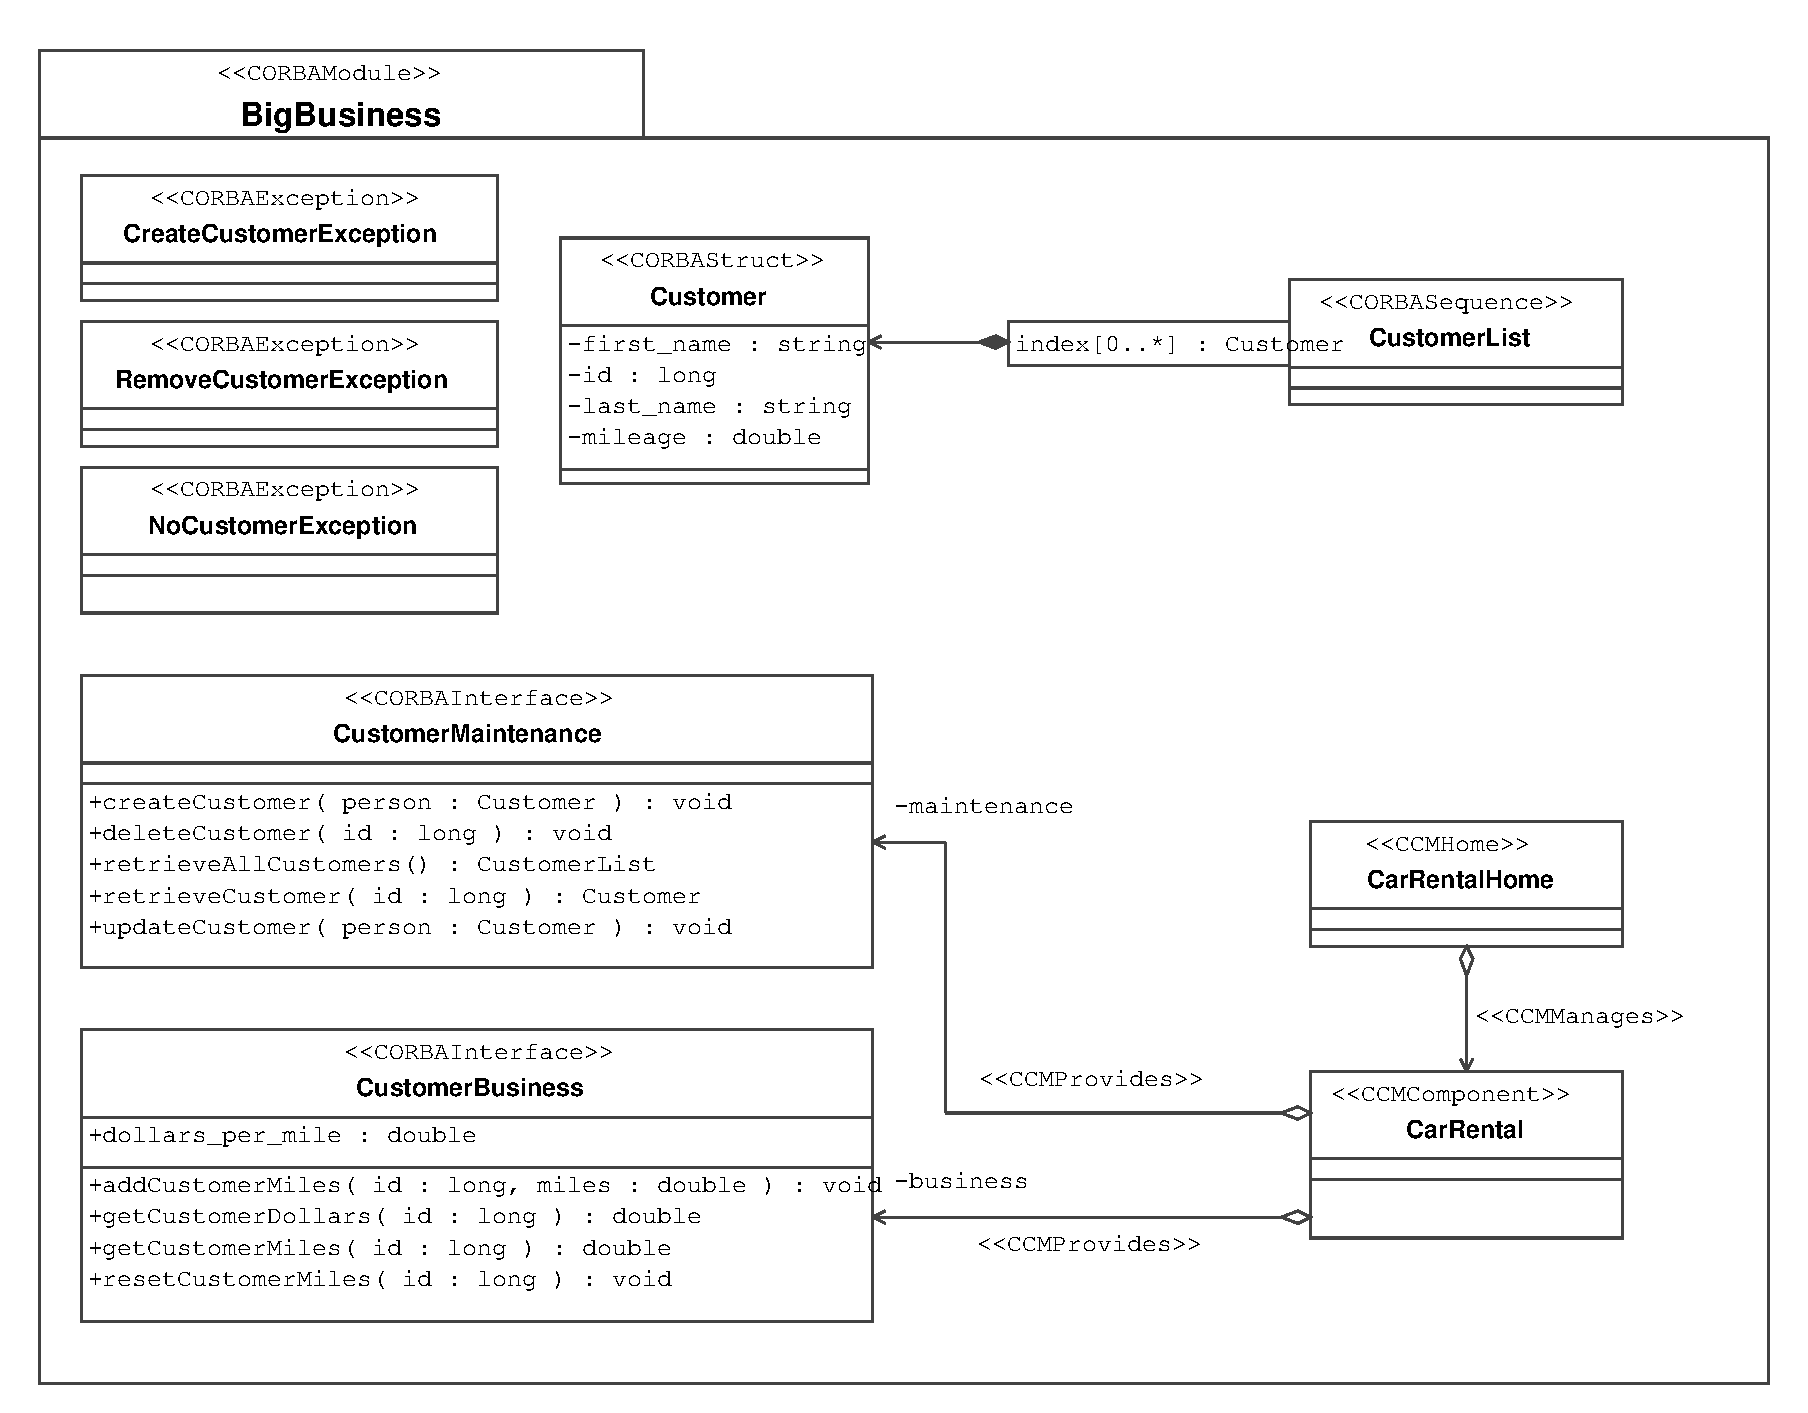
\includegraphics [width=13cm,angle=0] {uml/Example1}
        \caption{CarRental component in UML}
        \label{fig:uml-component-example}
    \end{center}
\end{figure}

We store the diagram (as an {\it XMI 1.1} file) in a directory called 
{\tt example2}, change to that directory and run the {\tt uml2idl} generator:
\begin{small}
\begin{verbatim}
    ~/example2> uml2idl uml/Example2.xml.zip example2
\end{verbatim}
\end{small}
After running {\tt uml2idl}, the new directory contains the following files:
\begin{small}
\begin{verbatim}
    example2/
    |-- example2.idl
    |-- example2.ocl
    `-- uml
        `-- Example2.xml.zip
\end{verbatim}
\end{small}

\newpage
\begin{itemize}
\item {\tt Example2.xml.zip}\\
This is the XMI file written from a UML tool.

\item {\tt example2.idl}\\ 
This file contains all generated IDL statements. 

\item {\tt example2.ocl} \\
In this file, all OCL expressions defined in the source model are stored.
Currently, we don't care about this file but we will use it in context of
Design by Contract. 
\end{itemize}

From the single IDL3 file, we generate a bunch of well structured 
IDL3 files as done with manually written files:
\begin{small}
\begin{verbatim}
    ~/example2> ccmtools-generate idl3 -o CarRental/idl3 *.idl
\end{verbatim}
\end{small}

Again, we have separated interfaces from component definitions:
\begin{small}
\begin{verbatim}
CarRental
`-- idl3
    |-- component
    |   `-- BigBusiness
    |       |-- CarRental.idl
    |       |-- CarRentalHome.idl
    |       |-- CarRentalHome_mirror.idl
    |       `-- CarRental_mirror.idl
    `-- interface
        `-- BigBusiness
            |-- CreateCustomerException.idl
            |-- Customer.idl
            |-- CustomerBusiness.idl
            |-- CustomerList.idl
            |-- CustomerMaintenance.idl
            |-- NoCustomerException.idl
            `-- RemoveCustomerException.idl
\end{verbatim}
\end{small}

That's it, we have made the first step toward MDA! 

But remember, we have only generated a component's structural description from
a UML diagram. The generated IDL file is a pure syntax description, without 
any semantics.  


%------------------------------------------------------------------------------
\section{The developers's job}
%------------------------------------------------------------------------------

It's important to know, that a developer's job does not change whether a 
component is designed in UML or IDL.
In both cases, a developer starts from the IDL3 file structure as shown above.


%% $Id: ProgrammingModel.tex,v 1.2 2004/07/27 19:18:57 teiniker Exp $

%==============================================================================
\chapter{Component Programming Model}
%==============================================================================

%------------------------------------------------------------------------------
\section{Overview}
%------------------------------------------------------------------------------

After writing our first component, we are ready to learn more about the 
component programming model.
When we are talking about component based development, we have to realize that there 
are two different views on the same component:
\begin{itemize}
\item {\bf Client's view}: As shown in the last section, a client finds a component 
home, creates a component instance and uses operations provided by the component's facets.

\item {\bf Business logic's view}: To implement some business logic, the component
developer has to know the programming API of the used component model.
There is a contract between the written code and the component's runtime environment.
The component container provides a {\it context object} that allows the component
instance to get information about its environment. In the other direction, the
component implements {\it callback methods} that are called by the container if any
life--cycle event occurs.
\end{itemize}

\begin{figure}[htbp]
    \begin{center}
        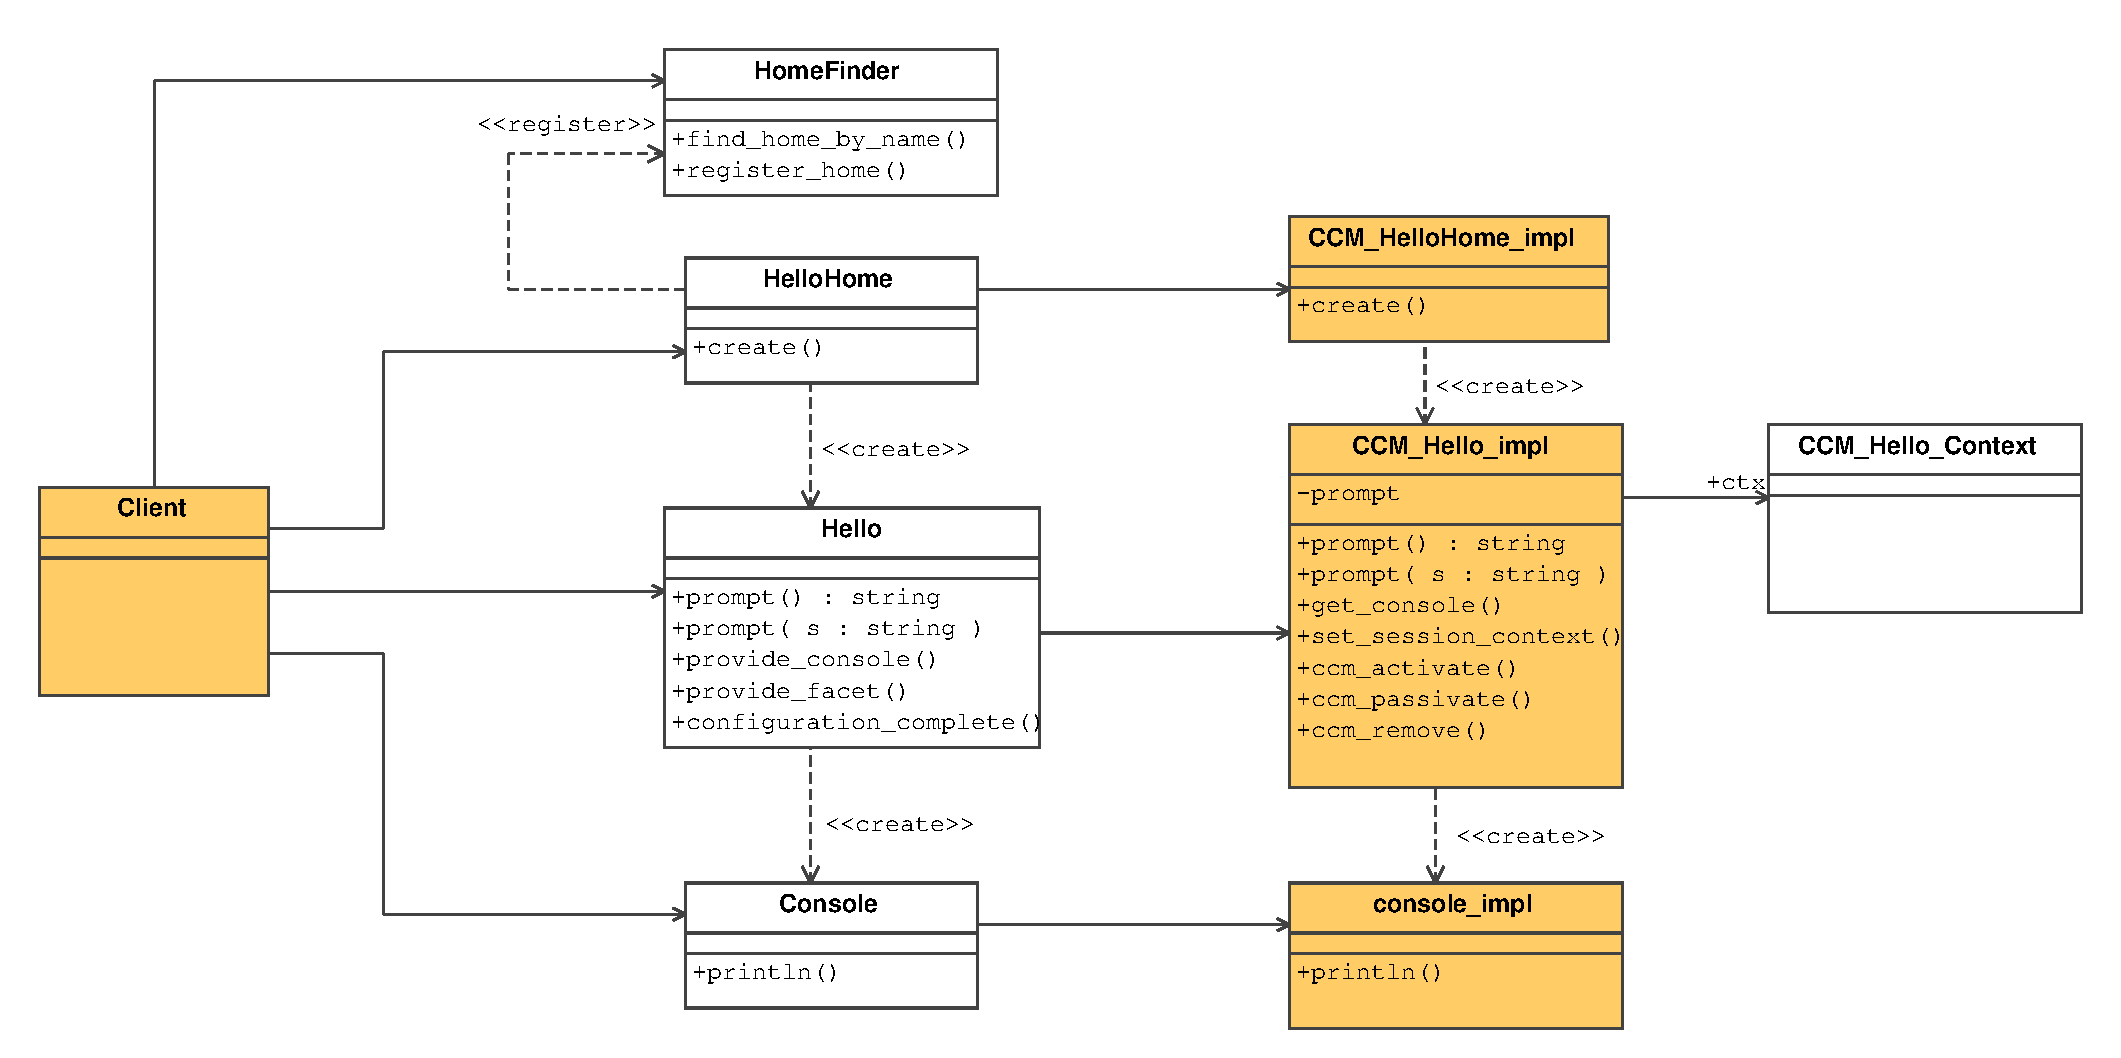
\includegraphics [width=12cm,angle=0] {uml/ComponentViews.eps}
        \caption{Client side and business logic view on the same component}
        \label{fig:ComponentViews}
    \end{center}
\end{figure}


%------------------------------------------------------------------------------
\section{Client's View}
%------------------------------------------------------------------------------

The client interacts with generated classes that are part of the component's
runtime environment. These adapter classes are generated from the definitions
in the IDL3 file.
Keep in mind, that a client never calls methods on the component's implementation
classes directly, every client call is intercepted by the component container. 

\begin{figure}[htbp]
    \begin{center}
        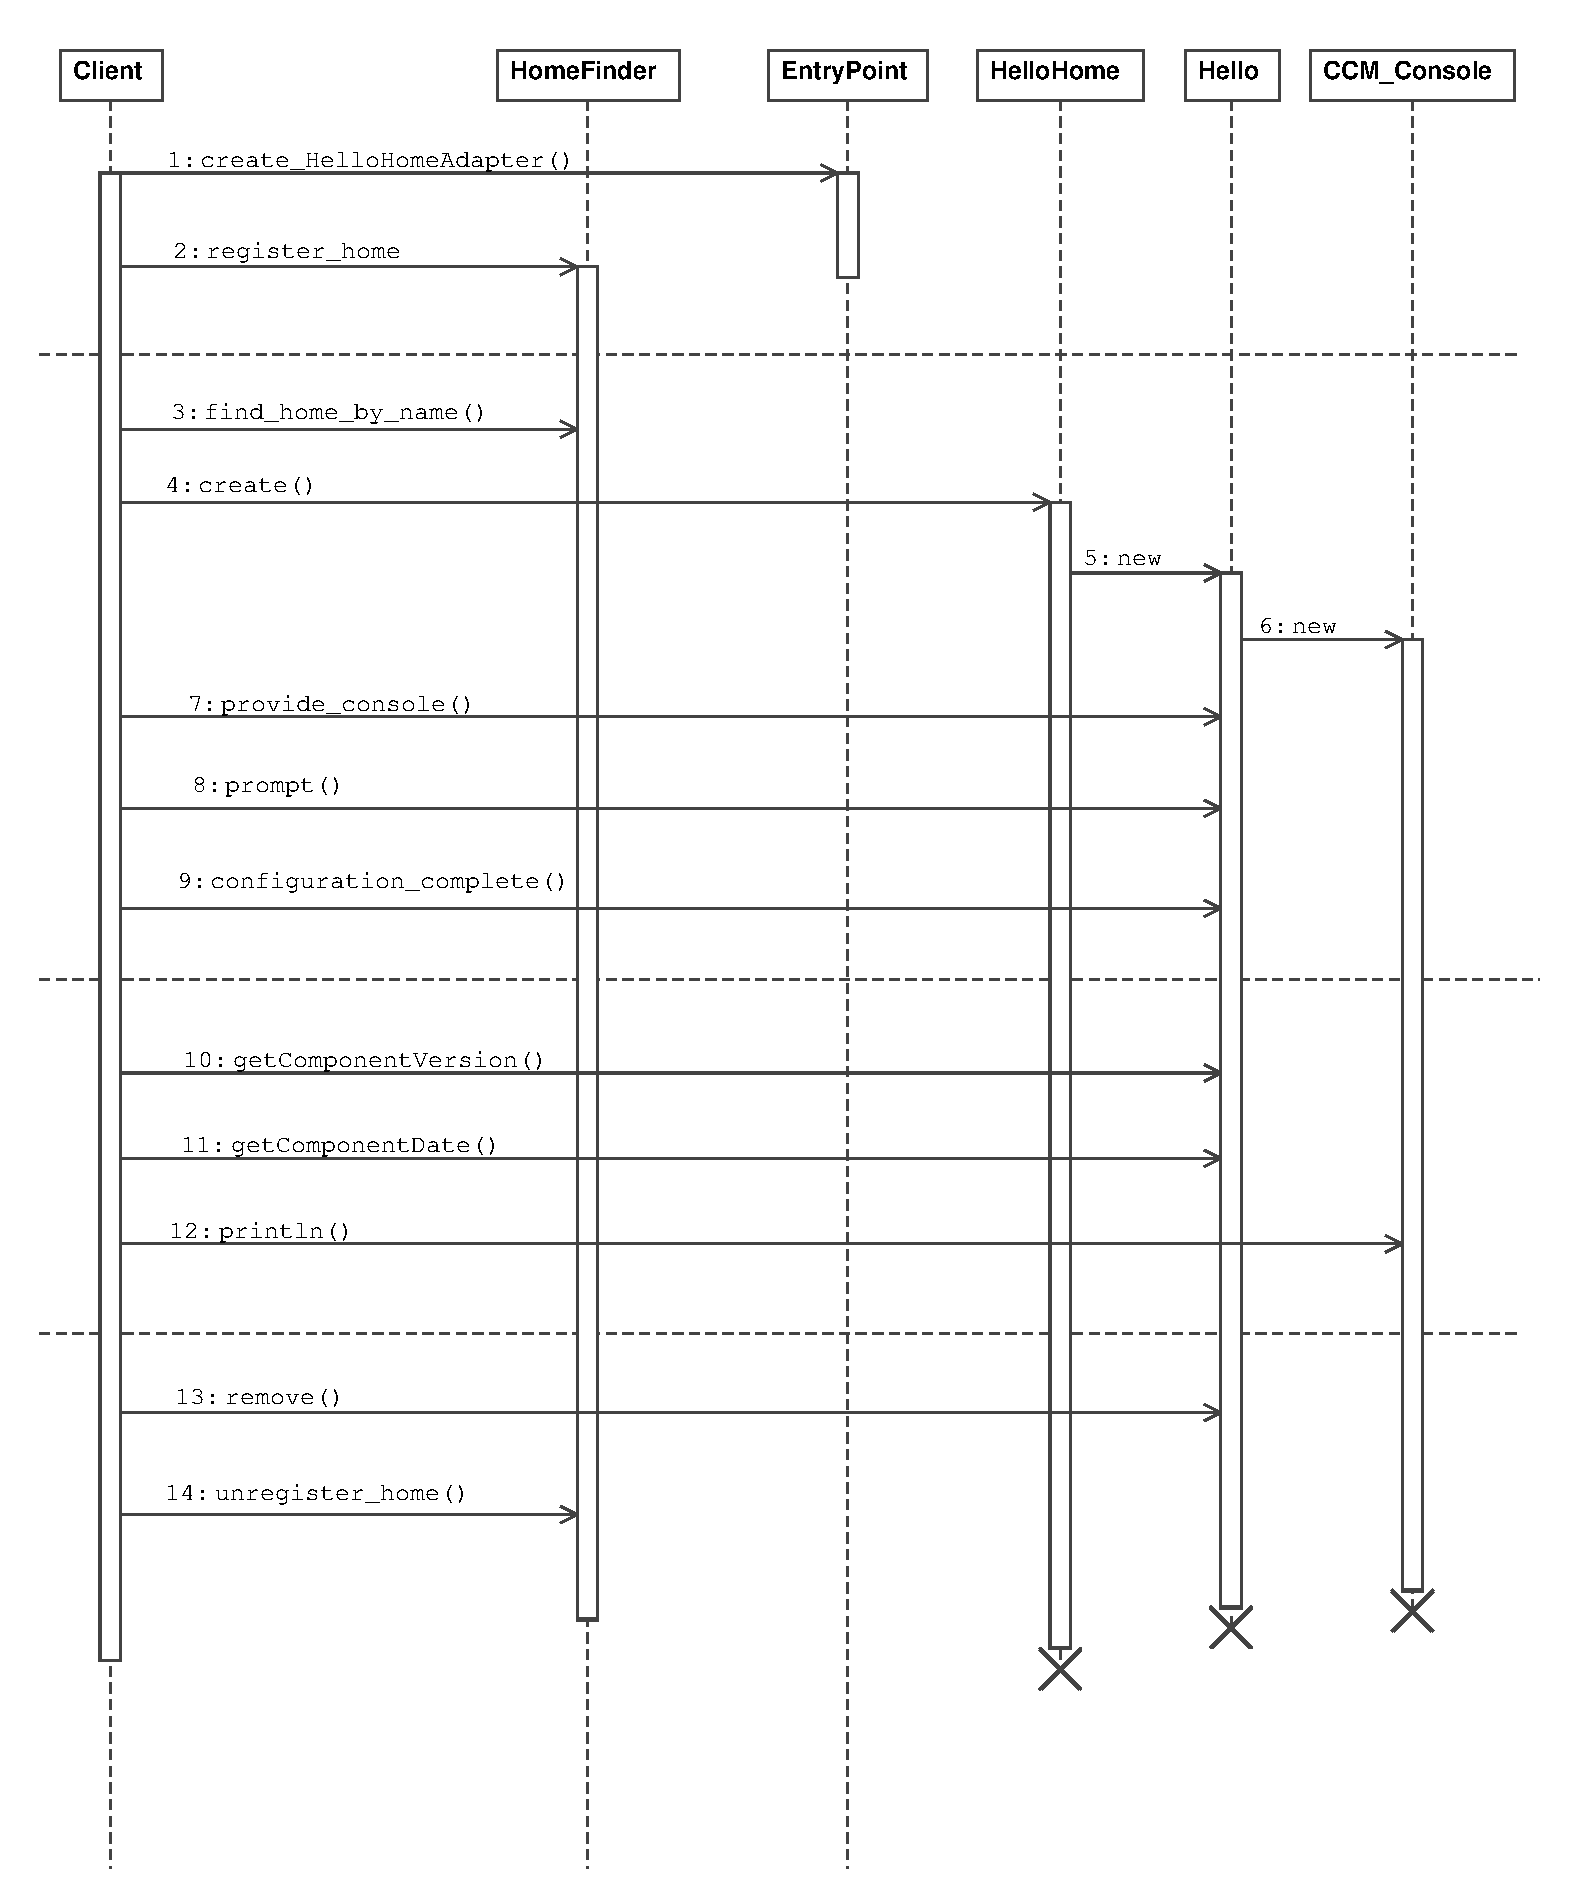
\includegraphics [height=16cm,angle=0] {uml/ClientView.eps}
        \caption{Client to component interaction}
        \label{ClientView}
    \end{center}
\end{figure}

\noindent
The related client code has been shown in the last chapter.
Note that the adapter classes are referenced via smart pointers. Therefore,
the adapters are deleted after their references go out of scope.


%------------------------------------------------------------------------------
\section{Business Logic's View}
%------------------------------------------------------------------------------

The component implementation only interacts with the component environment.
Each client call is delegated through the container to the implementation class.
The component's life--cycle is controlled by the container using callback methods.

\begin{figure}[htbp]
    \begin{center}
        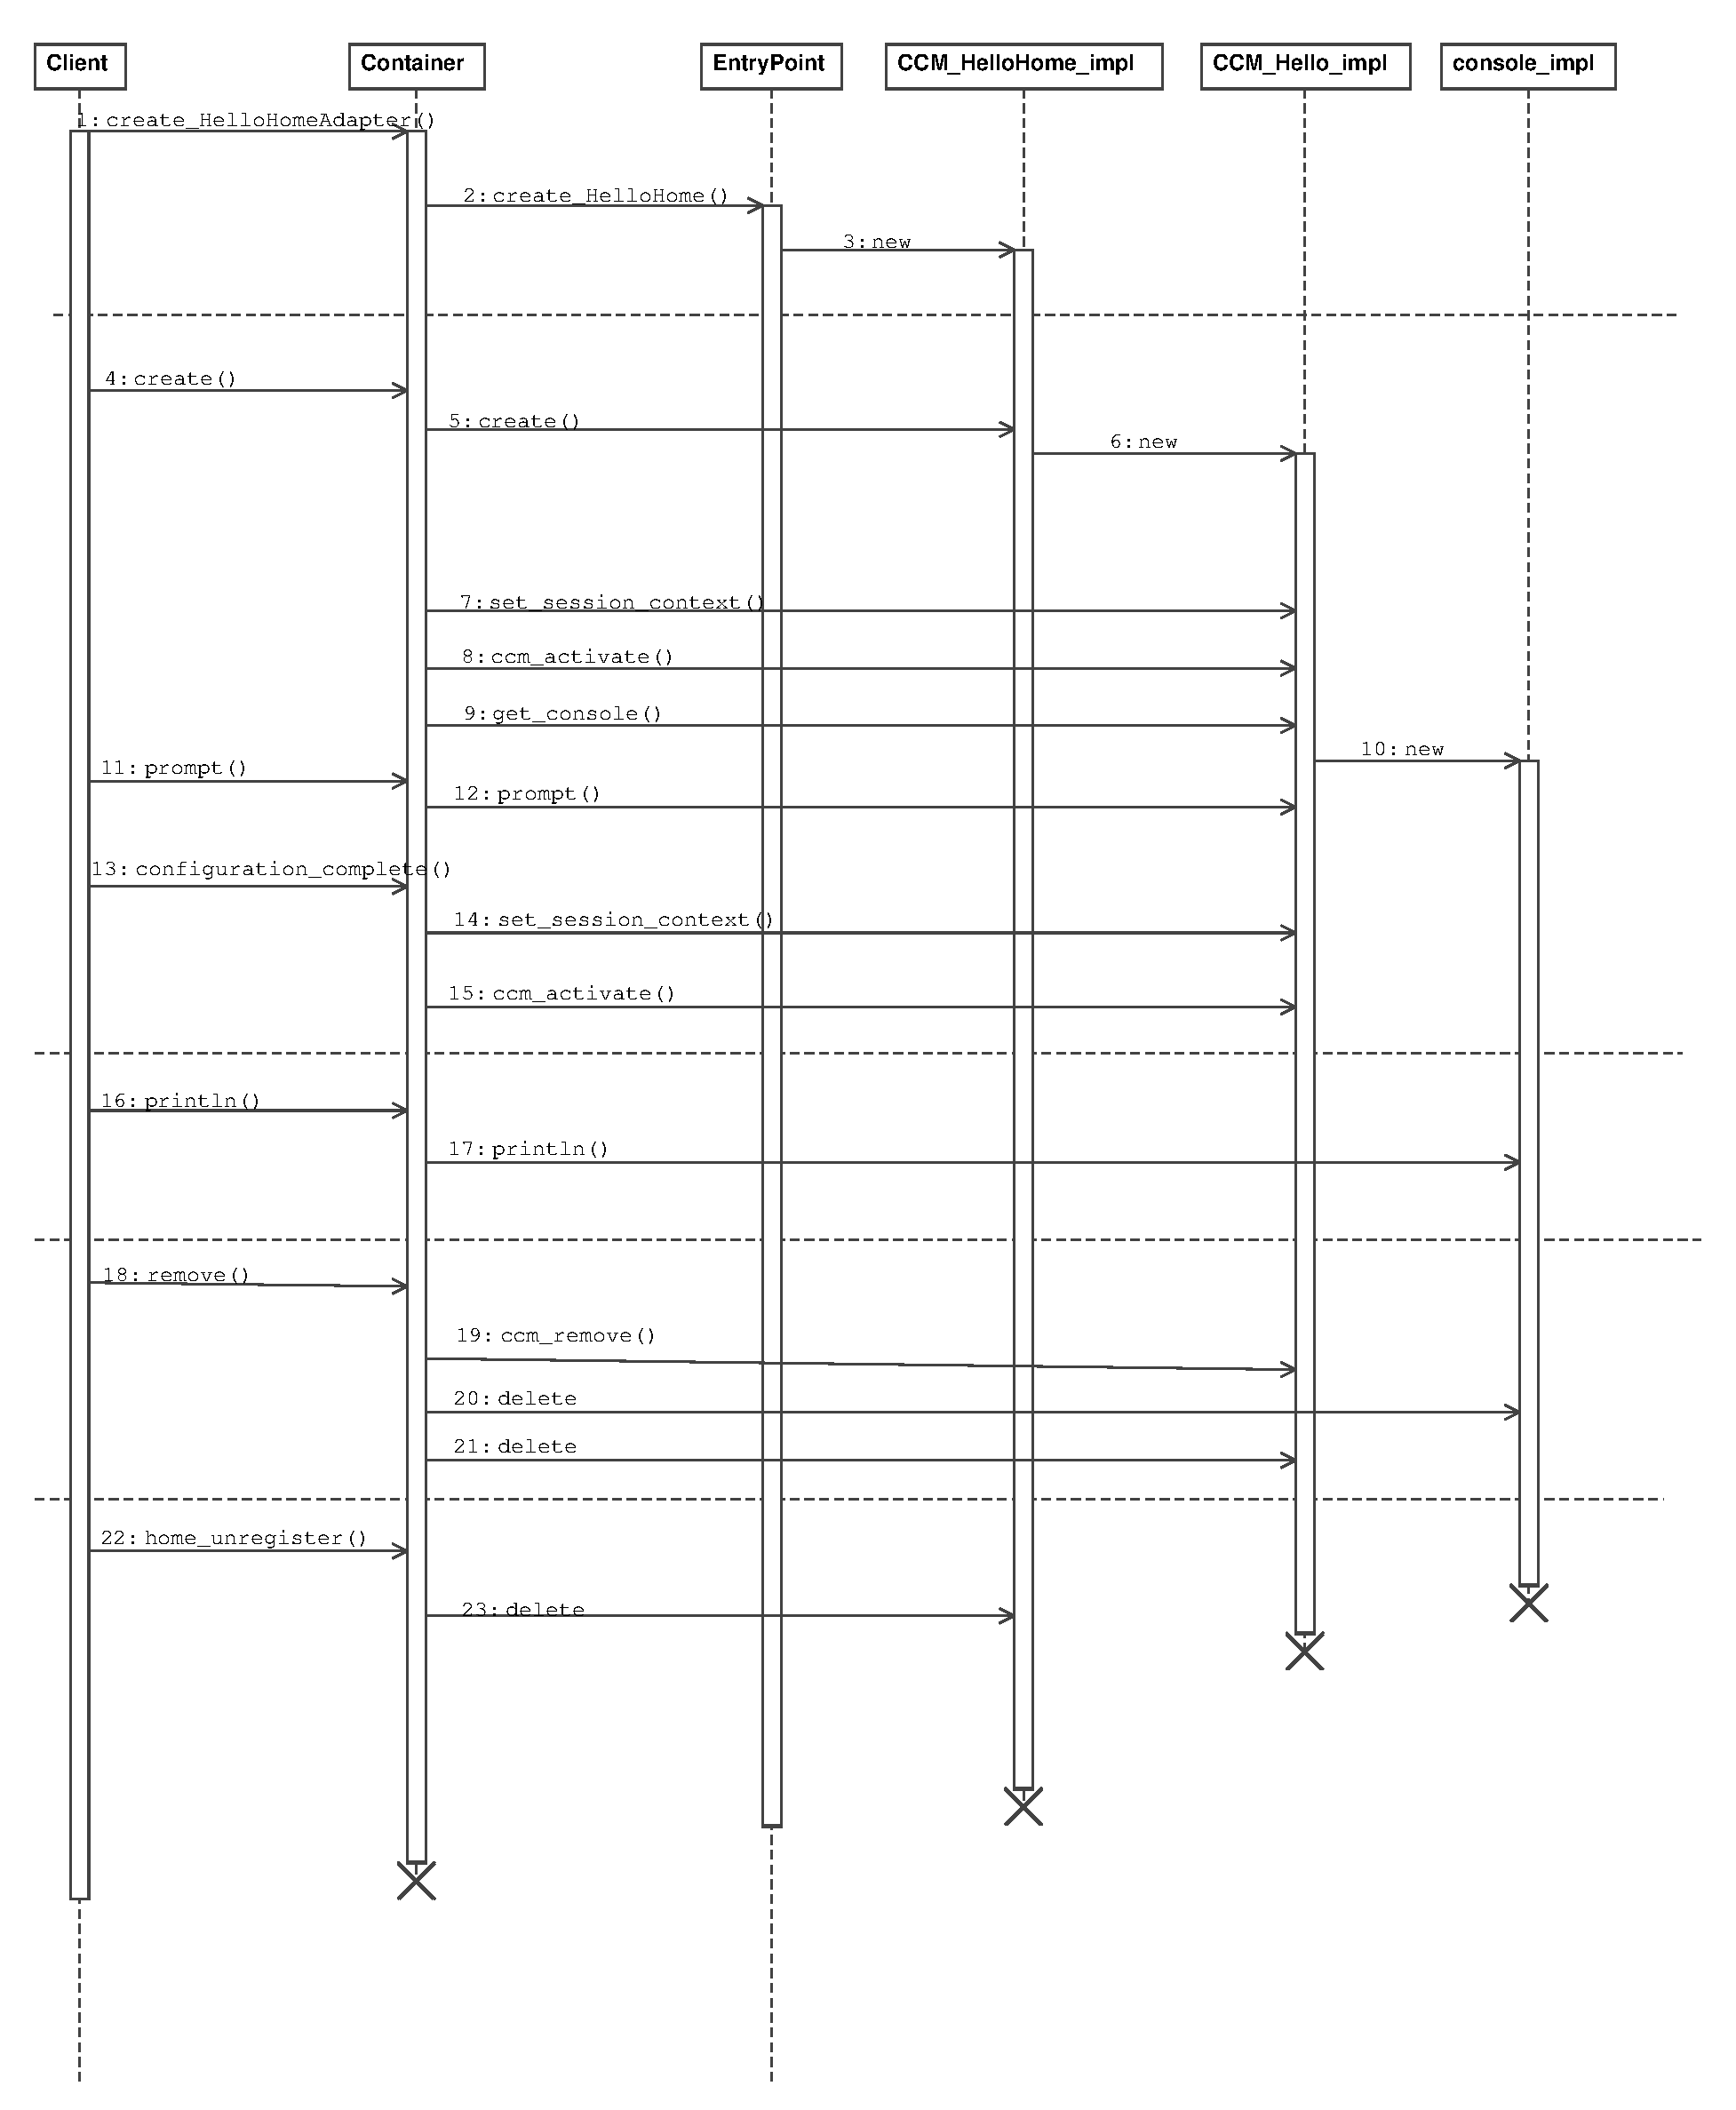
\includegraphics [height=17cm,angle=0] {uml/BusinessLogicView.eps}
        \caption{Container and component interaction}
        \label{BusinessLogicView}
    \end{center}
\end{figure}


With the following source code, we describe the classes that must be written to 
implement a component, as shown in figure \ref{fig:ComponentViews}.
Remember, the component developer only has to consider the contract between the
component and its container.

After writing the IDL3 file, we can hack the code that realizes the component's
home:
\begin{small}
\begin{verbatim}
/**
 * HelloHome_app.h file
 **/

#ifndef __HelloHome__APP__H__
#define __HelloHome__APP__H__
#include "HelloHome_gen.h"

namespace CCM_Local {
namespace CCM_Session_Hello {

class CCM_HelloHome_impl
  : public CCM_HelloHome
{
 public:
  virtual localComponents::EnterpriseComponent* create()
    throw (localComponents::CCMException);
};

} // /namespace CCM_Session_Hello
} // /namespace CCM_Local

extern "C" {
  localComponents::HomeExecutorBase* create_HelloHome();
}

#endif
\end{verbatim}
\end{small}

\begin{small}
\begin{verbatim}
/**
 * HelloHome_app.cc file
 **/

#include "HelloHome_app.h"

using namespace std; 
namespace CCM_Local {
namespace CCM_Session_Hello {

/**
 * The create() method instantiates a new component class and returns the
 * pointer to the container.
 * Note that the result is of type localComponents::EnterpriseComponent*
 * The container is responsible to delete the component class instance. 
 **/
localComponents::EnterpriseComponent* CCM_HelloHome_impl::create()
  throw (localComponents::CCMException)
{
  return dynamic_cast<localComponents::EnterpriseComponent*> (new CCM_Hello_impl());
}

} // /namespace CCM_Session_Hello
} // /namespace CCM_Local

/**
 * This is the entry point for the business logic. The container calls this
 * factory method to get a pointer to the home class implementation.
 * Note that the return value is of type localComponents::HomeExecutorBase*
 * The container is responsible to delete the home class instance.
 **/
extern "C" {
  localComponents::HomeExecutorBase* create_HelloHome()
  {
    return new CCM_Local::CCM_Session_Hello::CCM_HelloHome_impl();
  }
}
\end{verbatim}
\end{small}

\noindent
While the component home creates the instances of a component type, the component's 
business logic is coded within the component and the facet classes:

\begin{small}
\begin{verbatim}
/**
 * Hello_app.h file
 **/

#ifndef __Hello__APP__H__
#define __Hello__APP__H__

#include "Hello_gen.h"

namespace CCM_Local {
namespace CCM_Session_Hello {

class CCM_Hello_impl
  : public CCM_Hello
{
 private:
  std::string prompt_;

 public:
  CCM_Hello_Context* ctx;

  std::string prompt();
  void prompt(std::string value);

  CCM_Console* get_console();

  void set_session_context (localComponents::SessionContext* ctx)
    throw (localComponents::CCMException);
  void ccm_activate()
    throw (localComponents::CCMException);
  void ccm_passivate()
    throw (localComponents::CCMException);
  void ccm_remove()
    throw (localComponents::CCMException);
};


class console_impl
  : public CCM_Console
{
 private:
  CCM_Hello_impl* component;

 public:
  console_impl(CCM_Hello_impl* component_impl);
  long println(const std::string& s);
};

} // /namespace CCM_Session_Hello
} // /namespace CCM_Local

#endif
\end{verbatim}
\end{small}


\begin{small}
\begin{verbatim}
/**
 * Hello_app.cc file
 **/

#include <iostream>
#include "Hello_app.h"

using namespace std;
using namespace CCM_Utils;

namespace CCM_Local {
namespace CCM_Session_Hello {

/**
 * This method instantiates a facet class and returns the instance pointer
 * of type CCM_Console* to the container.
 * The container is responsible to delete the facet class instance.
 * Note that the name of the get_*() method corresponds with the facet name.
 **/
CCM_Console* CCM_Hello_impl::get_console()
{
  console_impl* facet = new console_impl(this);
  return dynamic_cast<CCM_Console*>(facet);
}

/**
 * This is the getter method for the prompt attribute.
 **/
std::string CCM_Hello_impl::prompt()
{
  return prompt_;
}

/**
 * This is the setter method of the prompt attribute.
 **/
void CCM_Hello_impl::prompt(const std::string value)
{
  prompt_ = value;
}

/**
 * Using this callback method, the container sets the session context, after
 * the client called configuration_complete().
 * The session context is used by the component to access receptacles and other
 * environment information.  
 **/
void CCM_Hello_impl::set_session_context(localComponents::SessionContext* context)
  throw (localComponents::CCMException)
{
  ctx = dynamic_cast<CCM_Hello_Context*>(context);
}

/**
 * The container calls this method after setting up the component instance.
 * In the same way as set_session_context(), this callback is triggered by the
 * client's configuration_complete() call.
 **/
void CCM_Hello_impl::ccm_activate()
  throw (localComponents::CCMException)
{}

/**
 * The container calls this method before the component instance will be
 * passivated.
 **/
void CCM_Hello_impl::ccm_passivate()
  throw (localComponents::CCMException)
{}

/**
 * The container calls this method before the component will be removed.
 * This call is triggered by the client calling the components remove() method.
 **/
void CCM_Hello_impl::ccm_remove()
  throw (localComponents::CCMException)
{}


/**
 * This is the constructor of the facet class. As parameter, we pass a pointer 
 * to the component instance. Using this pointer, the facet operations can
 * access the components attributes as well as the context object. 
 **/
console_impl::console_impl(CCM_Hello_impl* component_impl)
  : component(component_impl)
{}

/**
 * This is the only business method within this example.
 * It only prints out the received string and returns the number of 
 * printed characters.
 */
long console_impl::println(const std::string& s)
{
  cout << component->prompt() << s << endl;
  return s.length();
}

} // /namespace CCM_Session_Hello
} // /namespace CCM_Local
\end{verbatim}
\end{small}





%%==============================================================================
\chapter{Connecting Components by Facet and Receptacle}
%==============================================================================
\begin{flushright}
{\it }
\end{flushright}


%------------------------------------------------------------------------------
\section{Overview}
%------------------------------------------------------------------------------
The CORBA component model also defines the concept of receptacles that are
connection points for facet references.
This section describes an example that extends the previous example with
a {\tt Display} component which is connected to the {\tt Hello} component,
as shown in Fig.~\ref{ConnectComponents}.

\begin{figure}[htbp]
    \begin{center}
        \includegraphics [width=10cm,angle=0] {ConnectComponents}
        \caption{Connecting components}
        \label{ConnectComponents}
    \end{center}
\end{figure}

The test client uses the component's home to create component instances.
The component instances are used for configuration and to provide facets.
To connect the two component instances, the {\tt LCD} facet is connected to
the {\tt LCD} receptacle.
Finally, the test client calls operations on the {\tt Console} facet that
are delegated to the {\tt Display} component.


%------------------------------------------------------------------------------
\section{Definition of two components}
%------------------------------------------------------------------------------
We define a new component called {\tt Display} that provides an {\tt LCD}
interface as a facet.
The {\tt Hello} component uses the {\tt LCD} interface as an receptacle.
Note that a facet to receptacle connection can only be established when
both ports handle the same interface.

\begin{verbatim}
    interface LCD {
      void display_text(in string s);
    };

    component Display {
      attribute string prompt;
      provides LCD lcd;
    };

    home DisplayHome manages Display {
    };


    interface Console {
      long println(in string s2);
    };

    component Hello {
      provides Console console;
      uses LCD lcd;
    };

    home HelloHome manages Hello {
    };
\end{verbatim}

\noindent
As long as we define the components in the same file, we have the same file structure
as before:  
\begin{verbatim}
        hello/
        |-- Hello.idl
\end{verbatim}



%------------------------------------------------------------------------------
\section{Implementation of two components}
%------------------------------------------------------------------------------

We start with generating and building the empty components:
\begin{verbatim}
~/hello> ccmtools-c++-generate -c 1.0 -d -p hello1.0 Hello.idl
~/hello> ccmtools-c++-configure -p hello1.0
~/hello> ccmtools-c++-make -p hello1.0
\end{verbatim}

\noindent
For each of the components a mirror component has been generated as well as a
test client that connects every component with its mirror component and calls 
the component's operations - Test-Driven Development.

To make it short, we implemented the following methods in the business logic
of the {\tt Display} and the {\tt Hello} component:
\begin{verbatim}
// Display_app.cc
void
lcd_impl::display_text ( const std::string& s )
{
  DEBUGNL ( " lcd_impl->display_text ( s )" );
  cout << component->prompt() << s;
}

// Hello_app.cc
long
console_impl::println ( const std::string& s2 )
{
  DEBUGNL ( " console_impl->println ( s2 )" );
  component->ctx->get_connection_lcd().ptr()->display_text(s2);
  cout << endl;
  return s2.length();	
}
\end{verbatim}

\noindent
We build the components again and install them in the component repository:
\begin{verbatim}
~/hello> ccmtools-c++-make -p hello1.0
~/hello> ccmtools-c++-install -p hello1.0
\end{verbatim}



%------------------------------------------------------------------------------
\section{Write a local test client for two components}
%------------------------------------------------------------------------------

To show the use of both components in an application, we write a test client in the
following file structure:
\begin{verbatim}
    hello/
    |-- hello1.0/
    |-- test/
    |   |-- client/
    |   |   |-- client.cc 
\end{verbatim}

\noindent
The client starts with a lot of include and using namespace statements.
Note that the included header files reflect the used components.
\begin{small}
\begin{verbatim}
#include <localComponents/CCM.h>
#include <CCM_Local/HomeFinder.h>
#include <CCM_Utils/Debug.h>

#include <CCM_Local/CCM_Session_Display/Display_gen.h>
#include <CCM_Local/CCM_Session_Hello/Hello_gen.h>
#include <CCM_Local/CCM_Session_Display/DisplayHome_gen.h>
#include <CCM_Local/CCM_Session_Hello/HelloHome_gen.h>

using namespace std;
using namespace CCM_Utils;
using namespace CCM_Local;
using namespace CCM_Session_Display;
using namespace CCM_Session_Hello;
\end{verbatim}
\end{small}

\noindent
In the main function, after setting the debugging mode, 
both component homes are registered at the home finder.
\begin{small}
\begin{verbatim}
int main ( int argc, char *argv[] )
{
  // Set debugging mode
  Debug::set_global(true);

  // Get in instance of the local HomeFinder and register component homes
  localComponents::HomeFinder* homeFinder = HomeFinder::Instance (  );
  try {                       
    homeFinder->register_home( create_DisplayHomeAdapter(), "DisplayHome" );
    homeFinder->register_home( create_HelloHomeAdapter(), "HelloHome" );
  } catch ( ... )  {
    cout << "Aut'sch: when register homes!" << endl;
    return -1;
  }
\end{verbatim}
\end{small}

\noindent
Now, we can use the home finder to find the homes by name.
We create an instance of each component, get references the the component's
facets and connect the facet of {\tt Display} with the receptacle of {\tt Hello}.
Note that both ports are defined by the same {\tt LCD} interface.
\begin{small}
\begin{verbatim}
  try {
    // Find component home
    SmartPtr<DisplayHome> myDisplayHome (dynamic_cast<DisplayHome*>
      ( homeFinder->find_home_by_name ( "DisplayHome").ptr ()));
    SmartPtr<HelloHome> myHelloHome (dynamic_cast<HelloHome*>
      ( homeFinder->find_home_by_name ( "HelloHome").ptr ()));

    // Create component instance
    SmartPtr<Hello> myHello = myHelloHome.ptr()->create();
    SmartPtr<Display> myDisplay = myDisplayHome.ptr()->create();
 
    // Get facet references and connect facets to receptacles
    SmartPtr<CCM_Console> console = myHello.ptr()->provide_console();	
    SmartPtr<CCM_LCD> lcd = myDisplay.ptr()->provide_lcd();
    myHello.ptr()->connect_lcd(lcd);

    // Configure the component's attribute
    myDisplay.ptr()->prompt("-=> ");

    // Component configuration finished	
    myHello.ptr()->configuration_complete();
    myDisplay.ptr()->configuration_complete();
\end{verbatim}
\end{small}

\noindent
The test client has build an component assembly of two components in memory and
can use its functionality. 
\begin{small}
\begin{verbatim}  
    // Call operations on the component assembly
    cout << "Display Version = " 
         << myDisplay.ptr()->getComponentVersion()  << endl;
    cout << "Hello Version = "  
         << myHello.ptr()->getComponentVersion() << endl;

    console.ptr()->println("Hello from the client");
\end{verbatim}
\end{small}

\noindent
To tear the component assembly town, we disconnect the ports and 
remove the component instances from memory.
We also unregister the component's homes from the home finder.
\begin{small}	
\begin{verbatim}    
    // Disconnect component ports
    myHello.ptr()->disconnect_lcd();    

    // Destroy component instances
    myDisplay.ptr()->remove();
    myHello.ptr()->remove();

    // Unregister component homes
    homeFinder->unregister_home("DisplayHome");
    homeFinder->unregister_home("HelloHome");
  }
  catch ( localComponents::HomeNotFound ) {
    cout << "Aut'sch: can't find a home!" << endl;
    return -1;
  }
  catch ( ... )  {
    cout << "Aut'sch: there is something wrong!" << endl;
    return -1;
  }
  return 0;
}
\end{verbatim}
\end{small}

\noindent
We build the test client with {\tt Confix} and run the binary:
\begin{verbatim}
~/hello/test> confix.py --bootstrap --configure  \
                        --make --targets=install --profile=ccmtools
~/hello/test> test_client_client
\end{verbatim}

\noindent
Isn't it cool?\\
We have run a test client that uses two components which are connected via facet 
and receptacle to build a component assembly.
In the same way, we can create more complex assemblies that form a real
component based application as well.

Look at the printed debugging information to trace the execution thread of the
test client. We can also switch off the messages by setting the debugging mode
in the main function to {\tt false}.







%% $Id: RemoteComponent.tex,v 1.1 2003/12/12 18:48:27 teiniker Exp $

%==============================================================================
\chapter{Remote Components}
%==============================================================================

%------------------------------------------------------------------------------
\section{Overview}
%------------------------------------------------------------------------------

After implementing and using local components, let's have a look at remote
components. 
While the CCM specification describes only remote components that are
accessible from CORBA clients,  
the goal of CCM--Tools is to support local components that can be put 
transparently into remote CCM components.
You can connect remote components (generated by the CCM-Tools) with any other 
CCM components (e.g. components generated by MicoCCM).

\begin{figure}[!htb]
    \begin{center}
        \includegraphics [width=7cm,angle=0] {LCAC_Overview}
        \caption{Local component adapter}
        \label{LcacOverview}
    \end{center}
\end{figure}

\noindent
An existing local component can fit into a remote component using adapter
classes, as shown in figure \ref{LcacOverview}. For each CORBA interface
of a remote component a adapter delegates the method calls to the local 
equivalent.
To get more information about the {\bf Local Component Adapter Concept} (LCAC)
see the Appendix of this document.

%------------------------------------------------------------------------------
\section{The designer's job}
%------------------------------------------------------------------------------

Of course, developing remote CORBA components starts with an IDL file. In fact, the
IDL comes from the CORBA stuff, and has already been used for local component 
development. 
To generate a remote layer around a local component, we can use existing IDL
files.
  
\begin{Example}
\begin{minifbox}
\begin{small}
\begin{verbatim}
interface Console {
  long println(in string s);
};

component Hello {
  attribute string prompt;
  provides Console console;
};

home HelloHome manages Hello {
};
\end{verbatim}
\end{small}
\end{minifbox}
\caption{Reusing the local component's IDL definition}
\label{example:one-component-idl}
\end{Example}


%------------------------------------------------------------------------------
\section{The developer's job}
%------------------------------------------------------------------------------

The basic idea is that a component developer always implements a local component.
Business logic is implemented in respect to the local component's programming
model without any CORBA in mind (and code ;-).
Thus, we start with implementing a local component as shown before:
\begin{small}
\begin{verbatim}
~/hello> ccmtools-c++-generate -d -c 2.0 -p hello2.0 Hello.idl
~/hello> ccmtools-c++-configure -p hello2.0
~/hello> ccmtools-c++-make -p hello1.0
\end{verbatim}
\end{small}

We implement the component's test, write the business logic, run the test and so on.
Remember, this iterative programming style forces short turn around cycles that are
not possible in a pure CORBA component environment.



%------------------------------------------------------------------------------
\subsection{Set up remote component environment}
%------------------------------------------------------------------------------

The remote components need some libraries, header and IDL files to run. All these
stuff can be generated, compiled and installed, using the following script: 
\begin{small}
\begin{verbatim}
~/hello> ccmtools-c++remote-environment
\end{verbatim}
\end{small}
	
\noindent
Note that the CCM--Tools need the {\bf Mico ORB}, {\bf IDL compiler} and 
{\bf NameService} to generate, build and run remote components.

 

%------------------------------------------------------------------------------
\subsection{Create the remote layer}
%------------------------------------------------------------------------------

To add a remote layer to an existing local component, we have to generate the
CORBA stubs and remote component adapters that join the CORBA objects with the
local component implementation.
All this code is generated using the following script:

\begin{small}
\begin{verbatim}
~/hello> ccmtools-c++remote-generate -d -p hello1.0 Hello.idl
\end{verbatim}
\end{small}
The {\tt ccmtools-c++remote-generate} script accepts the following command line
parameters:
\begin{itemize}
\item {\tt -d, -\-debug }\\
Enable debugging in generated code. The generated code produces a lot of debug
messages that can be used to trace the program execution. This also causes a
test client to be generated.

\item {\tt -p NAME, -\-package=NAME}\\
Set package name to NAME. The default package name is ``ccmtools-package''. Note
that the package name is used for the name of the generated subdirectory, unless
you override this behavior with the {\tt -o} option.

\item {\tt -h, -\-help}\\
Print out a short description of the available command line parameters.
\end{itemize}


\noindent
Beside the already existing directories and files of the local component code, 
now there are some new directories that contains the code for CORBA stubs and 
the remote component adapters.
Additionally, a second test file ({\tt \_check\_CCM\_Session\_*\_remote.cc}) is
created.

\begin{small}
\begin{verbatim}
    hello/
    |-- Hello.idl
    |-- _check_CCM_Session_Hello_remote.cc
    |-- hello1.0/
    |   |-- CCM_Session_Hello_remote
    |   |-- CCM_Test
    |   |-- idl2
\end{verbatim}
\end{small}

\noindent
We can build the local component code as well as the remote code with the
following commands:
\begin{small}
\begin{verbatim}
~/hello> ccmtools-c++-configure -p hello1.0
~/hello> ccmtools-c++-make -p hello1.0
\end{verbatim}
\end{small}
After the configure and build process, the local and the remote component tests
are started.
For the remote component test we use the CORBA collocation mechanism. Thus the 
generator  can implement the server and client code in a single test file.
Remember that to run the remote test a CORBA NameService must be established.


%------------------------------------------------------------------------------
\subsection{Deploy the remote component}
%------------------------------------------------------------------------------

To install the generated remote component library and header files in the
component repository, we can use the known CCM--Tools script:
\begin{verbatim}
~/hello> ccmtools-c++-install -p hello1.0
\end{verbatim}

\noindent
Applications can use the repository to access local or remote components 
like ordinary libraries.


%------------------------------------------------------------------------------
\subsection{Write a remote client and server}
%------------------------------------------------------------------------------

A remote component must be activated within a CORBA server application that
includes the header files of the ORB, the CORBA stubs and the remote
component.
\begin{Example}
\begin{minifbox}
\begin{small}
\begin{verbatim}
#include <CORBA.h>
#include <coss/CosNaming.h>

#include <CCM_Utils/Debug.h>
#include <CCM_Remote/CCM_Session_Hello/HelloHome_remote.h>
#include <Hello.h>

using namespace std;
using namespace CCM_Utils;
\end{verbatim}
\end{small}
\end{minifbox}
\caption{CORBA and remote component header files.}
\label{ServerHeaderFiles}
\end{Example}

\noindent
The remote {\tt Hello} component can be activated using the generated {\tt deploy\_HelloHome()} 
function. The first parameter is the initialized ORB object and the second parameter
defines the name of the component's home. This name is used to register the component's
home in the CORBA NameService. 
\begin{Example}
\begin{minifbox}
\begin{small}
\begin{verbatim}
int main (int argc, char *argv[])
{
  // Set debugging mode
  Debug::set_global(true); 

  // Initialize ORB and value type factories
  CORBA::ORB_var orb = CORBA::ORB_init(argc, argv);
  CCM::register_all_factories (orb);

  int error = deploy_HelloHome(orb, "HelloHome:1.0");
  if(!error) {
    cout << "Component is running..." << endl;
  }
  else {
    cerr << "ERROR: Can't start components!" << endl;
    assert(0);
  }

  // Wait for CORBA requests
  orb.run();
}
\end{verbatim}
\end{small}
\end{minifbox}
\caption{Remote component activation.}
\label{RemoteComponentServer}
\end{Example}

\noindent
Note that the ORB must be initialized and started before a remote component
can be accessed from a CORBA client.

\noindent
The remote client also has to initialize the ORB and the CORBA NameService,
as shown in Example \ref{ClientInit}.
\begin{Example}
\begin{minifbox}
\begin{small}
\begin{verbatim}
int main (int argc, char *argv[])
{
  Debug::set_global(true); 

  // Initialize ORB 
  CORBA::ORB_var orb = CORBA::ORB_init(argc, argv);
  CORBA::Object_var obj = 
    orb->resolve_initial_references ("NameService");
  CosNaming::NamingContextExt_var nc = 
    CosNaming::NamingContextExt::_narrow (obj);
\end{verbatim}
\end{small}
\end{minifbox}
\caption{Initialize the client's ORB and NameService.}
\label{ClientInit}
\end{Example}

From the CORBA NameService, the client gets a reference to the 
remote component's home. 
After narrowing the CORBA reference to the particular home type, 
the {\tt create()} method is used to get a component instance.
From the component instance we get a {\tt Console} facet reference, 
and set the {\tt prompt} attribute. 
A {\tt configuration\_complete()} call finishes the component 
configuration.

\begin{Example}
\begin{minifbox}
\begin{small}
\begin{verbatim}
  // Find ComponentHomes in the Naming-Service
  obj = nc->resolve_str ("HelloHome:1.0");
  HelloHome_var myHelloHome = HelloHome::_narrow (obj);

  // Create component instances
  Hello_var myHello =  myHelloHome->create();

  // Provide facets   
  Console_var console = myHello->provide_console();
	
  // Configure the component's attribute
  myHello->prompt("=->");

  // Component configuration finished	
  myHello->configuration_complete();
\end{verbatim}
\end{small}
\end{minifbox}
\caption{Creating the remote component and facet.}
\label{CreatingRemoteComponent}
\end{Example}

\noindent 
Now the remote client can use the component instance to call methods on
the component's equivalent interface and the supported facet.
%Every client request is forwarded to a CORBA object on the server side
%that workes as an adapter to the local component implementation. 
\begin{Example}
\begin{minifbox}
\begin{small}
\begin{verbatim}
  // Call operations on the component and its facets
  cout << "Version = " << 
    myHello->getComponentVersion() << endl;
  cout << "Date = " << 
    myHello->getComponentDate() << endl;

  console->println("Hello from the remote client");
\end{verbatim}
\end{small}
\end{minifbox}
\caption{Calling the remote component methods.}
\label{RemoteMethodCalling}
\end{Example}

\noindent
Finally, the remote client removes the component instance on the server side
and exits from the main function.

\begin{Example}
\begin{minifbox}
\begin{small}
\begin{verbatim}
  // Destroy component instances
  myHello->remove();
}
\end{verbatim}
\end{small}
\end{minifbox}
\caption{Destroy component instance.}
\label{DestroyComponent}
\end{Example}



%------------------------------------------------------------------------------
\subsection{Undeploy the remote component}
%------------------------------------------------------------------------------

To remove the component's libraries and header files from the repository, 
call:
\begin{verbatim}
~/hello> ccmtools-c++-uninstall -p hello1.0
\end{verbatim}
Remember, only the installed libraries and header files are deleted while
the developers source code remains untouched.



%------------------------------------------------------------------------------
%\subsection{Remote component packaging}
%------------------------------------------------------------------------------


\begin{appendix}
%$Id: ManPage.tex,v 1.5 2004/07/27 20:16:11 teiniker Exp $

%==============================================================================
\chapter{CCM Tools Commands}
%==============================================================================

%------------------------------------------------------------------------------
\section{ccmtools-generate}
%------------------------------------------------------------------------------

\begin{description}

\item [NAME:] 
  {\tt ccmtools-generate} - Frontend to start available CCM Tools generators.

\item [SYNOPSIS:] 
  {\tt ccmtools-generate TYPE [OPTIONS] FILES}

\item [DESCRIPTION:]
The {\tt ccmtools-generate} script is used to run a particular component generator 
backend based on a set of IDL files. 
Depending on {\tt TYPE} and {\tt OPTIONS} a particular code generator is selected 
to create the desired output.

\item [TYPE:]
  Currently, the following generator types are supported:
  \begin{itemize}
  \item {\tt c++local}\\
    Generates local C++ component logic.
    
  \item {\tt c++local-test} \\
    Generates a test client for a pair of local C++ component and
    mirror component.
    
  \item {\tt c++dbc} \\
    Generates a set of Design by Contract adapters for a local
    C++ component.
    
  \item {\tt idl3 }\\
    Generates IDL3 source files.

  \item {\tt idl3mirror }\\
    Generates IDL3 source files for a mirror component.
    
  \item {\tt idl2} \\
    Generates equivalent IDL2 source files.

  \item {\tt c++remote} \\ 
    Generates a set of remote C++ adapters that establish a standard
    compliant CORBA component where a local C++ component can be embedded.

  \item {\tt c++remote-test}\\
    Generates a test client for a pair of remote component and mirror component.
  \end{itemize}
  
\item [OPTIONS:]
  In addition to the generator types, the {\tt ccmtools-generate} script handles
  the following options:
  \begin{itemize}
  \item {\tt -a, --application} \\
    Forces the local C++ generator to create business logic
    implementation skeletons ({\tt *\_impl.*} files).

  \item {\tt -h, --help} \\
    Prints out a short description of the available command line parameters.

  \item {\tt -Ipath} \\
    Specifies a path that will be handled from a preprocessor to find 
    included IDL files.

  \item {\tt -o DIR, --output=DIR} \\
    Specifies the directory where the generated code will be written. 

  \item {\tt -V, --version} \\
    Prints out the current version of installed CCM Tools.
  \end{itemize}
  
\item [FILES:]
  This {\tt ccmtools-generate} script can handle single IDL files or a list of IDL
  files. The following examples show the usage of IDL files: 
  \begin{verbatim}
    ccmtools-generate idl3mirror -o test/idl3mirror Test.idl
    ccmtools-generate c++local -a -o test Test.idl Helper.idl 
    ccmtools-generate c++local-test -o test *.idl
  \end{verbatim}
\item [SEE ALSO:]
\end{description}


%------------------------------------------------------------------------------
\section{ccmtools-idl}
%------------------------------------------------------------------------------

\begin{description}

\item [NAME:] 
  {\tt ccmtools-idl} - Run an IDL compiler to generate CORBA stub and skeletons.

\item [SYNOPSIS:] 
  {\tt ccmtools-idl OPTION FILES}

\item [DESCRIPTION:]
  The {\tt ccmtools-idl} script is a IDL compiler wrapper for Mico ORB and Java ORB,
  and hides the different call notations. This script also allows to process more than
  one IDL file at the same time. 
  Note that this script assumes that both IDL compilers are installed correctly.

\item [OPTION:]
  The {\tt ccmtools-idl} script supports of the following options:
  \begin{itemize}
  \item {\tt -h, --help} \\
    Prints out a short description of the available command line parameters.

  \item {\tt -Ipath} \\
    Specifies a path that will be handled from a preprocessor to find 
    included IDL files.
   
  \item {\tt --mico} \\
    Forces the use of Mico's IDL compiler.
    Thus, the generated stub and skeletons are implemented in C++.

  \item {\tt --java} \\
    Forces the use of Java's build in IDL compiler.
    Thus, the generated stub and skeletons are implemented in Java.
    Note that Java's IDL compiler only supports CORBA 2.x but no CORBA 3.0 extensions
    like {\tt component}, {\tt home}, etc.

  \item {\tt -V, --version} \\
    Prints out the current version of installed CCM Tools.
  \end{itemize}
  
\item [FILES:]
  This {\tt ccmtools-idl} script can handle single IDL files or a list of IDL
  files. The following examples show the usage of IDL files: 
  \begin{verbatim}
    ccmtools-idl --mico CarRental.idl
    ccmtools-idl --java CarRental.idl Customer.idl
    ccmtools-idl --mico *.idl
  \end{verbatim}

\item [SEE ALSO:]
  {\tt Mico manual, Java IDL documentation}
\end{description}


%------------------------------------------------------------------------------
\section{uml2idl}
%------------------------------------------------------------------------------

\begin{description}

\item [NAME:] 
  {\tt uml2idl} - Convert an UML XMI file into an IDL and an OCL file. 

\item [SYNOPSIS:] 
  {\tt uml2idl XMI-FILE PREFIX}

\item [DESCRIPTION:]
  The {\tt uml2idl} script runs a Java program that converts a UML diagram stored
  in an XMI 1.1 file into corresponding IDL and OCL files.
  The IDL file is created in respect to the {\it CCM Profile for CCM}, while the
  OCL file collects all OCL expressions defined in the UML diagram.

\item [XMI-FILE:]
  That's the name of the input XMI 1.1 file which holds the UML class diagram
  (e.g. when using MagicDraw, the file name looks like {\tt Name.xml.zip}).

\item [PREFIX:]
  The generated IDL and OCL files are named {\tt PREFIX.idl} and {\tt PREFIX.ocl}.

\item [SEE ALSO:]
  {\tt UML Profile for CORBA, UML Profile for CCM}
  
\end{description}

%==============================================================================
\chapter{Confix Installation}
%==============================================================================
\begin{flushright}
{\it }
\end{flushright}

%------------------------------------------------------------------------------
\section{Prerequisites}
%------------------------------------------------------------------------------
To install Confix, the following programs must be available:

\begin{itemize}
\item Python, at least version 2.1.3.
\item Automake, at least version 1.5.
\item Autoconf, at least version 2.52.
\item Libtool. Support for Libtool is optional in Confix, so you may leave
it out entirely. Version 1.4.3 has been reported to give occasional
errors, 1.4.2 and 1.5 are ok.
\end{itemize}


%------------------------------------------------------------------------------
\section{How to get it}
%------------------------------------------------------------------------------

The project's homepage it hosted on Sourceforge,
{\tt http://confix.sourceforge.net}. See there for releases,
announcements et cetera.

%------------------------------------------------------------------------------
\section{Source distribution}
%------------------------------------------------------------------------------
Unpack the file, point the {\tt PYTHONPATH} environment variable into
the root directory of the Confix package, and your {\tt PATH}
environment variable into the {\tt scripts} subdirectory thereof. For
example,
\begin{verbatim}
$ tar zxplf Confix-x.y.z.tar.gz
\end{verbatim}

Then make a call to Distutils to build and install the source.
\begin{verbatim}
$ cd Confix-1.0.1.tar.gz
$ pwd
/home/jfasch/Confix-1.0.1
$ python setup.py install --prefix=<confix_path>
\end{verbatim}

Then, provided the prefix you gave wasn't a standard one like
{\tt /usr} or {\tt /usr/local}, you should update your environment
accordingly. For example, you could add the following lines to your
{\tt ~/.bashrc},
\begin{verbatim}
PREFIX=<confix_path>
export PYTHONPATH=$PYTHONPATH:$PREFIX/lib/pythonA.B/site-packages
export PATH=$PATH:$PREFIX/bin
\end{verbatim}

Make sure A.B corresponds to the version of Python that you use, such
as 2.1 or 2.2.

%==============================================================================
\chapter{Mico Installation}
%==============================================================================
\begin{flushright}
{\it }
\end{flushright}

%------------------------------------------------------------------------------
\section{Prerequisites}
%------------------------------------------------------------------------------

Before trying to compile MICO make sure you have installed the following
software packages:
\begin{itemize}
\item make, at least version 3.7
\item gcc 2.95.x or gcc 3.2.x 
\end{itemize}


%------------------------------------------------------------------------------
\section{How to get it}
%------------------------------------------------------------------------------

The MICO homepage is found at
{\tt http://www.mico.org}. 


%------------------------------------------------------------------------------
\section{Source distribution}
%------------------------------------------------------------------------------

\begin{verbatim}
$ tar xvzf mico-2.3.10.tar.gz
$ cd mico
$ configure --prefix=<confix_path> 
$ make
$ make install
$ ldconfig -v
\end{verbatim}
\end{appendix}

%=References===================================================================
\bibliographystyle{plain}
\bibliography{./bibtex/cbse,./bibtex/doc,./bibtex/wx,./bibtex/pattern,./bibtex/se,./bibtex/mda}

\end{document}


